\documentclass[11pt,a4paper]{article}
\usepackage[text={6.5in,10in},centering,a4paper]{geometry}
\usepackage{indentfirst}
\usepackage{setspace}
\usepackage{amssymb,amsmath} % Equations
\usepackage{tabularx} % Tables
\usepackage{graphicx,color} % Graphics, Figures
\usepackage[tight,footnotesize]{subfigure}
\usepackage{pgfgantt} % for gantt chart
\usepackage[hidelinks]{hyperref}
\usepackage[titletoc]{appendix}
\usepackage[nottoc,numbib]{tocbibind}
\usepackage[numbers]{natbib}
\usepackage[no-math]{fontspec}
\usepackage{xunicode} % for Thai fonts
\usepackage{xltxtra} % for Thai fonts
\usepackage{circuitikz}
\usepackage{pgfplots}
\usepackage{tikz}
\usepackage{pdfpages}

\def\figurename{รูปที่}
\def\tablename{ตารางที่}
\def\refname{เอกสารอ้างอิง}
\def\chaptername{บทที่}
\def\abstractname{\large Abstract}
\def\contentsname{สารบัญ}
\def\listfigurename{สารบัญรูป}
\def\listtablename{สารบัญตาราง}
\def\figurename{รูป}
\def\tablename{ตาราง}
\def\appendixname{ภาคผนวก}

\graphicspath{{figures/}} % create a director 'figures' in your local dir and all pics are kept here

%========== Thai Font ===========================
\XeTeXlinebreaklocale "th_TH"
\defaultfontfeatures{Scale=1.0, Mapping=tex-text}
\setmainfont[Scale=1.2]{TH Sarabun New}
%========== Thai Font ===========================

%=========== Flowchart ==========================
% \tikzstyle(startstop) [rectangle,rounded corner, minimum width= 3cm]
%=========== Flowchart ==========================

\usetikzlibrary{math}

\begin{document}
\thispagestyle{empty}
\begin{center}
    \doublespacing
    {\LARGE \bf ข้อเสนอโครงงานวิศวกรรมไฟฟ้า วิชา 2102490}
    \vfill
    {
        \LARGE \bf
        % ชื่อโครงงานภาษาไทย
        อิเล็กทรอนิกส์กำลังสำหรับระบบเก็บเกี่ยวพลังงานชนิดเครื่องจักรกลไฟฟ้า \\[2ex]
        % ชื่อโครงงานภาษาอังกฤษ
        Power Electronics for Electromechanical Energy-Harvesting System
    }
    \vfill
    {\LARGE \bf นายณัฐพล กาบแก้ว เลขประจำตัว 6130176521}\\[2ex]
    {\LARGE \bf นายสันติ ว่องประเสริฐ เลขประจำตัว 6130553421}\\[2ex]
    {\LARGE \bf อาจารย์ที่ปรึกษา รศ.ดร. สุรพงศ์ สุวรรณกวิน}
    \vfill
    {\LARGE \bf ภาควิชาวิศวกรรมไฟฟ้า คณะวิศวกรรมศาสตร์}\\[2ex]
    {\LARGE \bf จุฬาลงกรณ์มหาวิทยาลัย}\\[2ex]
    {\LARGE \bf ปีการศึกษา 2564}
\end{center}

\newpage
\thispagestyle{empty}
\tableofcontents

\newpage
\setcounter{page}{1}
\section{บทนำ}
\subsection{บทคัดย่อ}
% add other commercial product details
แผ่นพื้นเก็บเกี่ยวพลังงานด้วยเครื่องจักรกลไฟฟ้าได้ถูกพัฒนาขึ้น โดยมีความสามารถในการจ่ายกำลังไฟฟ้าให้กับอุปกรณ์ที่ใช้พลังงานต่ำได้ โครงงานฉบับนี้ มีจุดประสงค์ในการพัฒนาแผ่นพื้นเก็บเกี่ยวพลังงานด้วยเครื่องจักรกลไฟฟ้าซิงโครนัส ประเภทแม่เหล็กถาวร (Permanent Magnet Synchronous Motor) โดยใช้โปรแกรม MATLAB\textsuperscript{TM}/Simulink\textsuperscript{TM} โดยโปรแกรม จะช่วยในการทดสอบ (Test) ทวนสอบ (Verify) ออกแบบให้ได้ผลดีที่สุด (Optimize design) และใช้โปรแกรมในการสร้างโค๊ดภาษาซี และซีพลัสพลัส ที่ถูกออกแบบสำหรับระบบฝังตัว (Generate C/C++ Code Optimized for Embedded Systems)  จากแบบจำลองที่ได้ออกแบบไว้ และใช้เทคนิคในการลดกำลังสูญเสียในอินเวอร์เตอร์ คืออัลกอริทึมในการมอดูเลตแบบสองแขน (Two Arm Modulation Algorithm) และการติดตามการทำงานในจตุภาคที่หนึ่ง (First Quadrant Tracking Algorithm) และได้เพิ่มประสิทธิภาพของระบบโดยรวมด้วยการนำอัลกอริทึมในการติดตามจุดทำงานที่ให้กำลังสูงสุด (Maximum Power Point Tracking Algorithm; MPPT ) มาใช้งาน

\subsection{ที่มาและความสำคัญของโครงงาน}
การเก็บเกี่ยวพลังงานจากการเคลื่อนไหวของมนุษย์นั้น เป็นเรื่องที่น่าสนใจ สามารถนำมาทำให้เกิดขึ้นจริงได้ และได้มีการศึกษามาแล้วในหลายๆ ครั้ง \cite{biomech} \cite{GpH:01} ซึ่งในการศึกษาดังกล่าว ได้ค้นพบว่า พลังงานที่ได้ในแต่ละการเหยียบแต่ละครั้งนั้น มีค่าน้อยมาก นั่นคือประมาณ 1-5 จูล เท่านั้น ดังนั้น หัวใจในการเก็บเกี่ยวพลังงานจากระบบดังกล่าว คือการมีประสิทธิภาพที่ดี จึงจะสามารถเก็บพลังงานได้เพียงพอกับการใช้งานต่อไป ดังนั้น การศึกษาในโครงงานฉบับนี้ จึงได้มุ่งเน้นในการเพิ่มประสิทธิภาพให้กับระบบเก็บพลังงานเป็นหลัก

แผ่นพื้นเก็บพลังงานนั้น ประกอบไปด้วยหลายส่วนที่สำคัญคือ ชิ้นส่วนเชิงกล บอร์ดอินเวอร์เตอร์ มอเตอร์ไฟฟ้า และระบบควบคุมที่อยู่ในระบบฝังตัว ดังที่แสดงไว้ในรูปที่ \ref{genpathtopology}
\begin{figure}[!h]
    \centering
    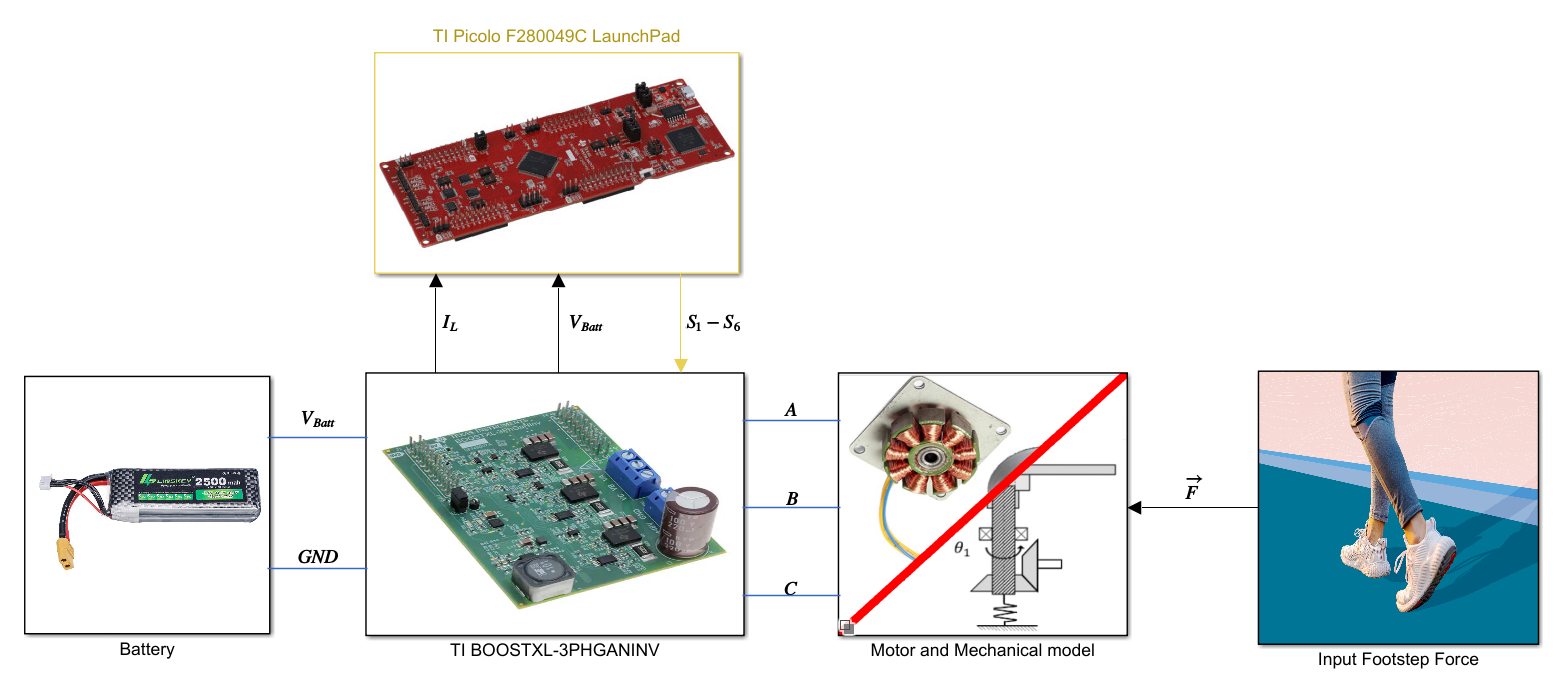
\includegraphics[width=\textwidth]{genpath_topology.png}
    \caption{ทอพอโลยีของระบบแผ่นพื้นเก็บพลังงาน}
    \label{genpathtopology}
\end{figure}

ในส่วนของอุปกรณ์เชิงกลของแผ่นพื้นเก็บพลังงานนั้น เนื่องจากโครงงานฉบับนี้ จะให้น้ำหนักกับการวิเคราะห์และออกแบบระบบไฟฟ้าเป็นสำคัญ จึงได้มีการนำอุปกรณ์เชิงกลที่ได้มีการวิเคราะห์และออกแบบไว้แล้วในโครงงานวิศวกรรมในปีก่อนๆ \cite{GpH:01} มาใช้งาน

\subsection{วัตถุประสงค์ของโครงงาน}
\begin{enumerate}
    \item เพื่อศึกษาแบบจำลองทางคณิตศาสตร์และสร้างแบบจำลองพลวัตของระบบแผ่นพื้นเก็บพลังงานด้วยโปรแกรม MATLAB\textsuperscript{TM}/Simulink\textsuperscript{TM} เพื่อตรวจสอบผลลัพธ์ที่ได้ก่อนนำไปใช้กับอุปกรณ์จริง
    \item เพื่อหาแนวทางในการลดพลังงานสูญเสียในระบบขับเคลื่อนเครื่องจักรกลไฟฟ้าซิงโครนัสประเภทแม่เหล็กถาวร และพัฒนาชุดอัลกอริทึมในการเพิ่มประสิทธิภาพให้กับระบบแผ่นพื้นเก็บพลังงาน
    \item เพื่อสร้างต้นแบบอุปกรณ์ แผ่นพื้นเก็บพลังงาน ที่สามารถใช้งานได้จริง

\end{enumerate}
% วัตถุประสงค์ คือผลลัพธ์สุดท้าย (Outcome) ของโครงงาน วัตถุประสงค์จะคล้ายกับหัวข้อโครงงาน เพียงแต่มีรายละเอียดและความชัดเจนมากกว่าหัวข้อ วัตถุประสงค์ควรเล็งถึงสิ่งที่เป็นรูปธรรม เช่น ออกแบบและสร้างอุปกรณ์ (Device) ประดิษฐ์หรือหาระเบียบวิธี (Algorithm) หาพารามิเตอร์หรือสภาวะที่เหมาะสม (Characterization or Optimization) ออกแบบและสร้างระบบ (System Integration) ศึกษาและเปรียบเทียบ (Study and Comparison) พัฒนาซอฟต์แวร์ (Software Development) วัตถุประสงค์ไม่ควรเป็นเพียงการกระทำ (Actions) ของนิสิต เช่น เรียนรู้การใช้โปรแกรม MATLAB/Simulink ศึกษาการใช้งานไมโครโปรเซสเซอร์ ทำความเข้าใจคณิตศาสตร์ เรียนรู้การใช้งานและทดสอบเครื่องมือ เป็นต้น นิสิตควรเขียนวัตถุประสงค์ให้กระชับ ไม่ควรยาวเกินหกบรรทัด และสามารถแยกเป็นข้อๆ เพื่อความชัดเจนได้ (ไม่ควรเกินสามข้อ) เช่น


% ตัวอย่างวัตถุประสงค์ของโครงงานหัวข้อ “การวิเคราะห์ผลกระทบของระบบผลิตไฟฟ้าจากพลังงานแสงอาทิตย์ที่มีต่อเสถียรภาพชั่วครู่ของระบบไมโครกริด”
% \begin{enumerate}
%     \item เพื่อวิเคราะห์ผลของระบบผลิตไฟฟ้าจากพลังงานแสงอาทิตย์ที่มีต่อเสถียรภาพชั่วครู่ของไมโครกริด ทั้งในสภาวะที่เชื่อมต่อกับกริดภายนอกและสภาวะแยกโดด
%     \item เพื่อวิเคราะห์ปัญหาเสถียรภาพชั่วครู่ของไมโครกริดเมื่อเกิดการรบกวนขนาดใหญ่ขึ้นในระบบ
% \end{enumerate}

% รายละเอียดในส่วนวัตถุประสงค์โครงงานในวิชา 2102499 นั้นจะต้องตรงกับที่เสนอไว้ในข้อเสนอโครงงานวิชา 2102490 ทุกประการ ถ้าหากในระหว่างการสอบข้อเสนอโครงงาน คณะกรรมการได้มีความเห็นให้เพิ่ม ลด แก้ไข หรือเปลี่ยนแปลงวัตถุประสงค์ นิสิตก็จะต้องจะแก้ไขตามคำแนะนำของคณะกรรมการด้วย
\newpage
\subsection{ขอบเขตของโครงงาน}
\begin{enumerate}
    \item โครงงานฉบับนี้จะใช้เครื่องจักรกลไฟฟ้าชนิดแม่เหล็กถาวร เป็นตัวกำเนิดไฟฟ้า
    \item โครงงานฉบับนี้จะใช้ไมโครคอนโทรลเลอร์ TI\textsuperscript{TM} F280049C ที่อยู่บนชุดทดลอง Picolo\textsuperscript{TM} LaunchPad\textsuperscript{TM} เป็นระบบฝังตัวแกนกลางในคำนวนอัลกอริทึมต่างๆ
    \item โครงงานฉบับนี้จะใช้บอร์ดอินเวอร์เตอร์ TI\textsuperscript{TM} BOOSTXL-3PHGaNINV เป็นสวิตช์สำหรับวงจรอินเวอร์เตอร์
    \item โครงงานฉบับนี้จะโปรแกรมระบบฝังตัวดังกล่าวผ่านการสร้างโค๊ดบนแพลตฟอร์ม Simulink\textsuperscript{TM} Embedded Coder\textsuperscript{TM}
\end{enumerate}
% ขอบเขตของโครงงานไม่ใช่ภาพรวมของโครงงาน ดังเช่นในวัตถุประสงค์ แต่เป็นการบอกเงื่อนไข สภาวะแวดล้อมที่ถูกสมมุติขึ้นสำหรับปัญหา รวมถึงผลลัพธ์ที่คาดหวังว่า จะมีขอบเขตอย่างไรที่วัดได้ โดยแยกเป็นข้อๆ แต่ละข้อต้องเป็นรูปธรรมที่ชัดเจน และต้องสามารถชี้วัดได้ในเชิงปริมาณไม่ใช่เชิงคุณภาพ เช่น เร็ว ควรเปลี่ยนเป็น อัตราอย่างน้อย 20 bps มีประสิทธิภาพสูง ควรเปลี่ยนเป็น ประสิทธิภาพอย่างน้อย 60 เปอร์เซ็นต์ เป็นต้น
% ตัวอย่างขอบเขตของโครงงาน


% ตัวอย่างขอบเขตของโครงงานหัวข้อ “เครื่องตรวจจับระดับความเป็นกรดด่างของน้ำในสระว่ายน้ำ”
% \begin{enumerate}
%     \item ใช้หลักการตรวจจับการเปลี่ยนแปลงความเข้มแสงย่านแสงสีแดง
%     \item สามารถใช้กับสระว่ายน้ำที่ต้องเติมคลอรีน ที่มีขนาดไม่เกิน 400 ลบ.ลิตร
%     \item สามารถวัดค่าความเป็นกรดด่างได้ในช่วง pH 6.5-7.5 โดยมีความผิดพลาดไม่เกิน ±0.05
%     \item สามารถตรวจจับได้อย่างรวดเร็ว โดยมีเวลาตอบสนองไม่เกิน 2 ms
% \end{enumerate}

% ขอบเขตของโครงงานในรายงานวิชา 2102499 นั้นจะต้องตรงกับที่เสนอไว้ในข้อเสนอโครงงานวิชา 2102490 โดยนิสิตสามารถเพิ่มขอบเขตได้ แต่ห้ามลดลง หากในระหว่างการสอบข้อเสนอโครงงาน คณะกรรมการได้มีความเห็นให้เพิ่ม ลด แก้ไข หรือเปลี่ยนแปลงขอบเขต นิสิตก็จะต้องแก้ไขตามคำแนะนำของคณะกรรมการด้วย

\subsection{ผลลัพธ์ที่คาดหวังจากโครงงาน}

% ให้นิสิตอธิบายถึงผลลัพธ์ที่เป็นรูปธรรมที่ชัดเจนจากการทำโครงงานนี้ โดยเลือกเฉพาะผลลัพธ์ที่เด่นและเป็นผลลัพธ์หลัก เช่น

\begin{enumerate}
    \item แผ่นพื้นเก็บพลังงานต้นแบบที่มีประสิทธิภาพสูง และสามารถใช้งานได้จริง
    \item อัลกอริทึมในการลดกำลังสูญเสียในอินเวอร์เตอร์ ที่สามารถนำไปใช้กับระบบแผ่นพื้นเก็บพลังงาน และยังสามารถนำไปใช้กับอินเวอร์เตอร์ใดๆ นอกเหนือจากระบบแผ่นพื้นเก็บพลังงานได้อีกด้วย
    \item อัลกอริทึมในการติดตามจุดทำงาน ที่ให้กำลังไฟฟ้าสูงสุด ที่สามารถนำไปใช้กับระบบแผ่นพื้นเก็บพลังงาน
\end{enumerate}

% ตัวอย่างผลลัพธ์ที่คาดหวังจากโครงงานหัวข้อ “การจำลองระบบทดสอบสำหรับใช้ศึกษาปัญหาเสถียรภาพชั่วครู่ในระบบส่งไฟฟ้ากำลัง”


% ระบบทดสอบที่สามารถนำไปใช้ศึกษาและวิเคราะห์ปัญหาเสถียรภาพชั่วครู่ได้อย่างถูกต้อง


% ผลลัพธ์ของโครงงานในวิชา 2102499 จะต้องตรงกับที่เสนอไว้ในข้อเสนอโครงงานวิชา 2102490 ห้ามลดมาตรฐานลง ถ้าในระหว่างการสอบข้อเสนอโครงงาน คณะกรรมการได้มีความเห็นให้ปรับปรุงผลลัพธ์ของโครงงาน นิสิตก็จะต้องแก้ไขตามความเห็นของคณะกรรมการด้วย

\section{หลักการและทฤษฎีที่เกี่ยวข้อง}

\subsection{การลดกำลังสูญเสียในอินเวอร์เตอร์ ด้วยอัลกอริทึมการมอดูเลตแบบสองแขน และการติดตามการทำงานในจตุภาคที่หนึ่ง (Two Arm Modulation and First Quadrant Tracking Algorithm)}

\subsubsection{การมอดูเลตความกว้างพัลส์แบบใช้สัญญาณพาหะ และ อินเวอร์เตอร์โหมดแรงดันแบบสามเฟส}
ในการขับเคลื่อนเครื่องจักรกลไฟฟ้าโดยทั่วไปนั้นอาศัยการสร้างสนามแม่เหล็กหมุน มาเหนี่ยวนำให้เกิดแรงบิด ซึ่งในกรณีของเครื่องจักรกลไฟฟ้าซิงโครนัสแบบแม่เหล็กถาวรนั้นอาศัยการสร้างสนามแม่เหล็กหมุนโดยใช้ไฟฟ้ากระแสสลับ อินเวอร์เตอร์ จึงเป็นอุปกรณ์ที่จำเป็นต่อระบบขับเคลื่อนเครื่องจักรกลไฟฟ้าซิงโครนัสแบบแม่เหล็กถาวรด้วยแหล่งจ่ายไฟฟ้ากระแสตรง ในโครงงานฉบับนี้ ได้นำเครื่องจักรกลไฟฟ้าซิงโครนัสแบบแม่เหล็กถาวรสามเฟส มาเป็นเครื่องกำเนิดไฟฟ้า สำหรับระบบแผ่นพื้นเก็บพลังงาน โดยจะเก็บพลังงานที่ผลิตได้ไว้กับแบตเตอร์รี ในโครงงานฉบับนี้ จึงเลือกใช้อินเวอร์เตอร์สามเฟสที่มีทอพอโลยีดังรูปที่ \ref{3phaseinv}
\begin{figure}[!h]
    \centering
    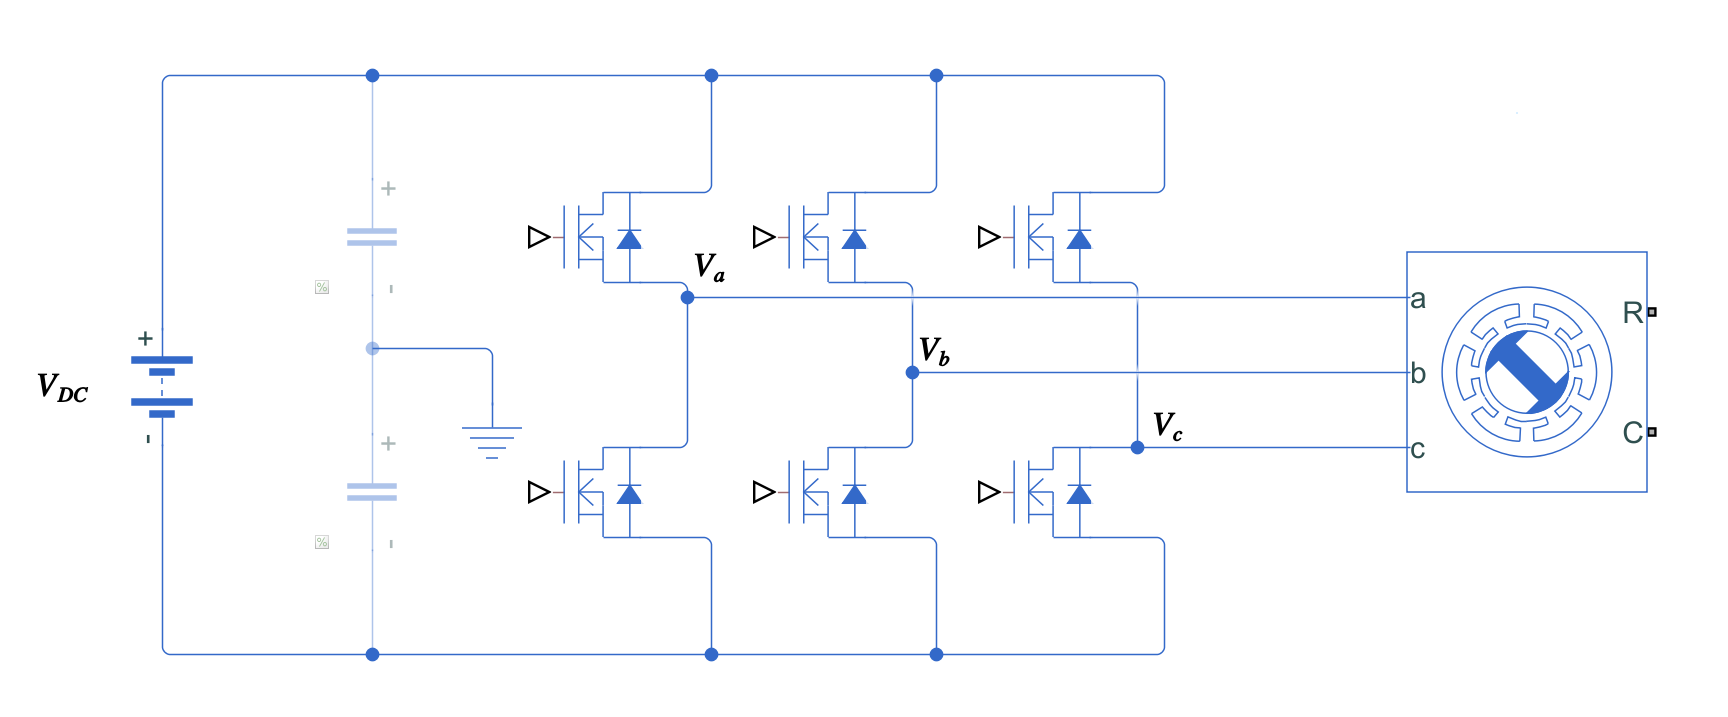
\includegraphics[width=\textwidth]{inverter_topology.png}
    \caption{ทอพอโลยีของอินเวอร์เตอร์สามเฟส}
    \label{3phaseinv}
\end{figure}

อินเวอร์เตอร์ทอพอโลยีที่ได้นำเสนอมาข้างต้น สามารถสร้างแรงดันออกที่แต่ละขั้วทั้งสามได้เพียงแค่ 2 ค่าเท่านั้นคือ
\begin{equation}
    V_t = \begin{cases}
        V_{DC}, & \text{ถ้าสวิตช์ตัวบนปิด และสวิตช์ตัวล่างเปิด} \\
        0,      & \text{ถ้าสวิตช์ตัวบนปิด และสวิตช์ตัวล่างเปิด}
    \end{cases}
\end{equation}
โดยที่ $V_t$ เป็นแรงดันที่ขั้วออกของอินเวอร์เตอร์
และถ้าหากพิจารณาให้กึ่งกลางบัสแรงดันไฟฟ้ากระแสตรงเป็นจุดอ้างอิงแรงดัน จะได้ว่า
\begin{equation}
    V_{t0} = \begin{cases}
        V_{DC}/2,  & \text{ถ้าสวิตช์ตัวบนปิด และสวิตช์ตัวล่างเปิด} \\
        -V_{DC}/2, & \text{ถ้าสวิตช์ตัวบนปิด และสวิตช์ตัวล่างเปิด}
    \end{cases}
\end{equation}

เนื่องจากกระขับเคลื่อนเครื่องจักรกลไฟฟ้าซิงโครนัสสามเฟสประเภทแม่เหล็กถาวรนั้น จำเป็นต้องใช้ไฟฟ้ากระแสสลับคลื่นรูปไซน์ ดังนั้น เทคนิคการมอดูเลตความกว้างพัลส์โดยใช้สัญญาณพาหะ (Carrier-based Pulse Width Modulation) จึงได้ถูกนำมาใช้ โดยการมอดูเลตความกว้างพัลส์โดยใช้สัญญาณพาหะมีหลักการในการทำงานคือ นำสัญญาณพาหะรูปสามเหลี่ยม มาเปรียบเทียบกับสัญญาณคำสั่ง โดยผลลัพธ์ของการเปรียบเทียบนั้น จะได้เป็นสัญญาณขับนำของสวิตช์ ดังรูปที่ \ref{spwmgraph} ซึ่งจะส่งผลให้ แรงดันที่ขั้วของอินเวอร์เตอร์ มีค่าเฉลี่ยเท่ากับแรงดันคำสั่ง

\begin{figure}[!h]
    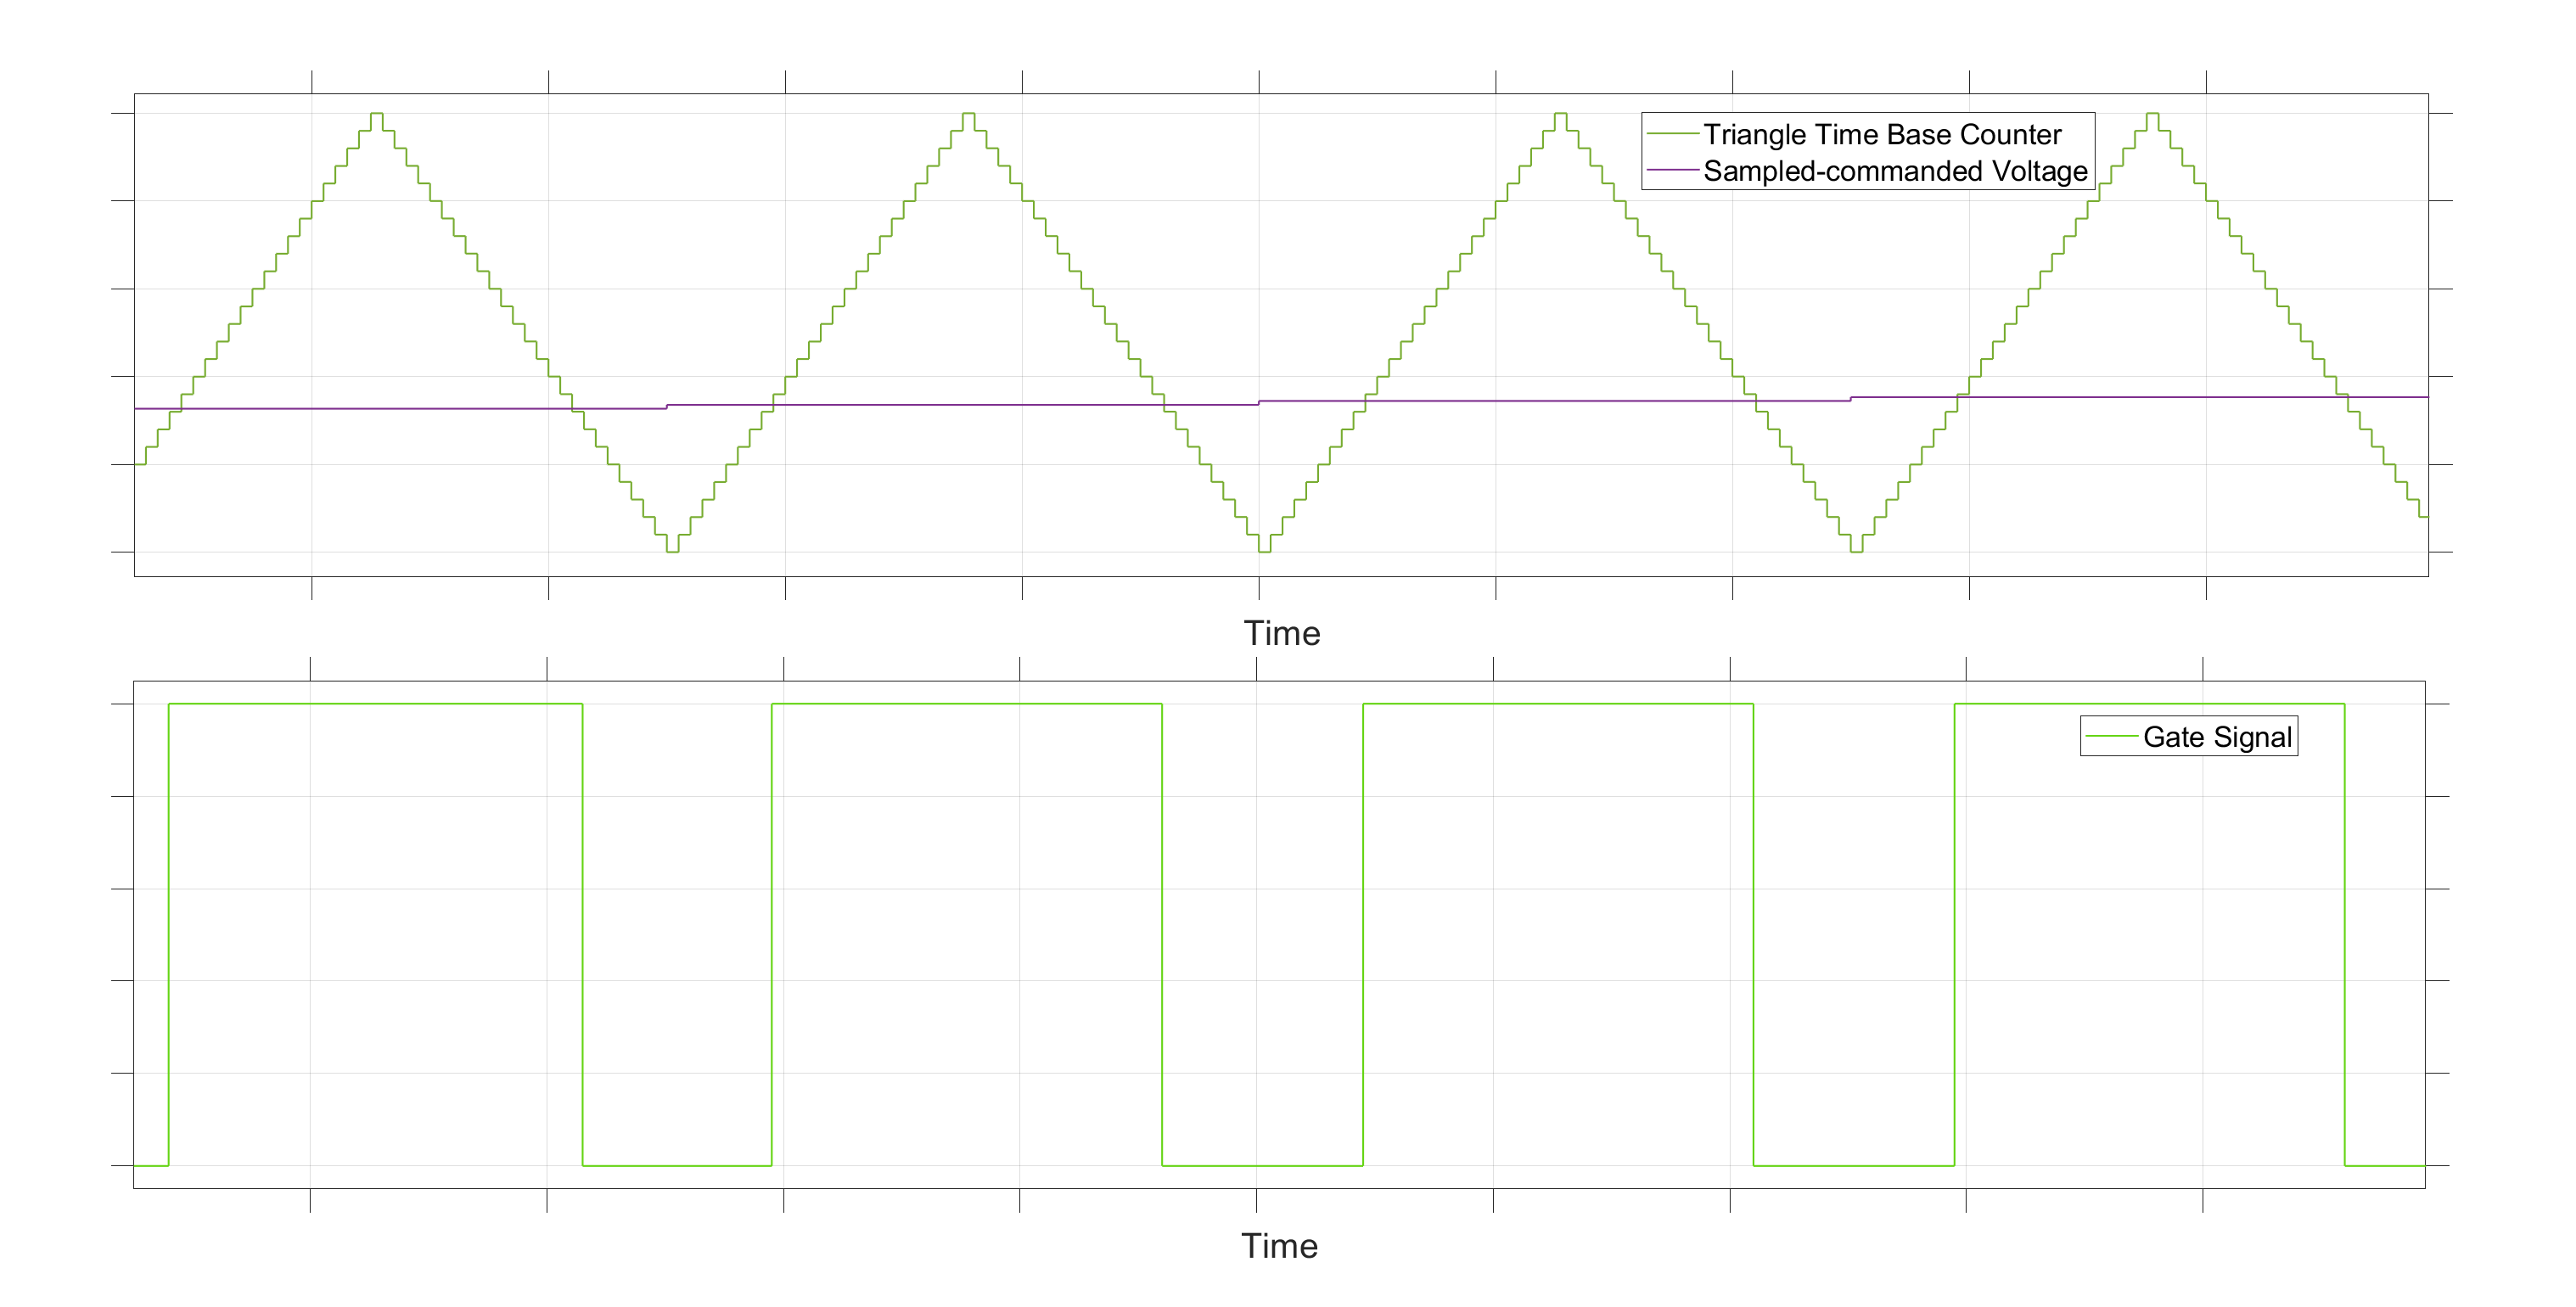
\includegraphics[width=\textwidth]{spwm.eps}
    \label{spwmgraph}
    \caption{การมอดูเลตความกว้างพัลส์โดยใช้สัญญาณพาหะ}
\end{figure}

จากรูปข้างต้น จะเห็นได้ว่าความกว้างพัลส์ของสัญญาณขับนำนั้น เปลี่ยนไปตามขนาดของสัญญาณคำสั่ง และสัญญาณที่จะนำมาเปรียบเทียบนั้น จะเป็นสัญญาณที่ถูกสุ่มตัวอย่างแล้วคงค่า (Sample and Hold) เพราะว่า อัลกอริทึมการมอดูเลตที่เลือกใช้ในโครงงานฉบับนี้นั้น เป็นการคำนวนบนระบบฝังตัว ซึ่งเป็นตัวประมวลผลในโดเมนดิจิทัล

\subsubsection{กำลังสูญเสียในสวิตช์ของอินเวอร์เตอร์}
กำลังสูญเสียในสวิตช์ของอินเวอร์เตอร์มีอยู่ด้วยกันสองประเภท คือ กำลังสูญเสียระหว่างสวิตช์ (Switching Loss) และกำลังสูญเสียระหว่างนำกระแส (Conduction Loss)
\begin{equation}
    P_{loss} = P_{sw} + P_{cond}
\end{equation}

\begin{figure}[h]
    \begin{center}
        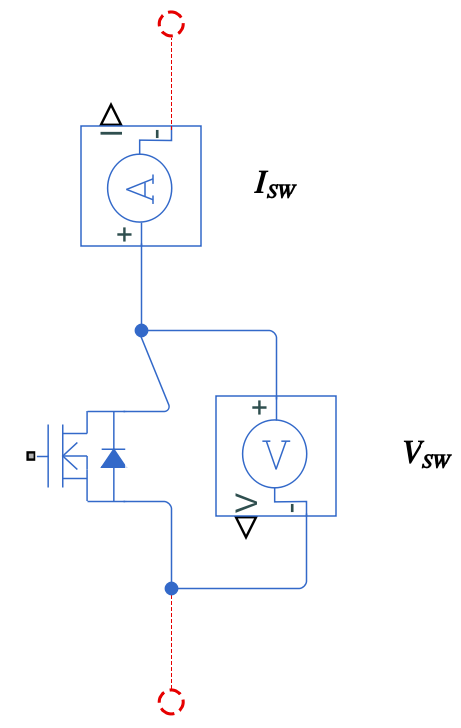
\includegraphics[width=0.25\textwidth]{vsw_isw.png}
    \end{center}
    \caption{นิยามของ $V_{SW}, I_{SW}$}
    \label{vsw_isw_definition}
\end{figure}

\begin{figure}[h!]
    \begin{center}
        \begin{tikzpicture}
            \pgfplotsset{width=\textwidth,height=\textwidth/3}
            \begin{axis}[
                    axis x line=middle,
                    axis y line=middle,
                    xlabel=$Time$,
                    xmax=45,
                    ymax=25,
                    ytick=\empty,
                    xtick=\empty,
                    xlabel near ticks,
                    xmin=0,
                    ymin=0,
                    every axis plot/.append style={ultra thick}
                ]
                % Plots
                \draw[fill=pink,opacity=0.2] (axis cs:2,0) rectangle (axis cs:10,25);
                \node at (axis cs:6,22) {\tiny $Switch-On$ $Region$};
                \draw[fill=green,opacity=0.2] (axis cs:10,0) rectangle (axis cs:25,25);
                \node at (axis cs:18,22) {\tiny $Conduction$ $Region$};
                \draw[fill=pink,opacity=0.2] (axis cs:25,0) rectangle (axis cs:32,25);
                \node at (axis cs:29,22) {\tiny $Switch-Off$ $Region$};
                \addplot[color=red] coordinates {(0,20) (5,20) (10,1) (25,1) (30,20) (35,20)};
                \addplot[color=blue] coordinates {(0,0) (2,0) (8,15) (27,15) (32,0) (35,0)};
                \legend{\tiny $V_{SW}$,\tiny $I_{SW}$}
            \end{axis}
        \end{tikzpicture}
        \begin{tikzpicture}
            \pgfplotsset{width=\textwidth,height=\textwidth/3}
            \begin{axis}[
                    axis x line=middle,
                    axis y line=middle,
                    xlabel=$Time$,
                    xmax=45,
                    ymax=25,
                    ytick=\empty,
                    xtick=\empty,
                    xlabel near ticks,
                    xmin=0,
                    ymin=0,
                    every axis plot/.append style={ultra thick}
                ]
                % Plots
                \draw[fill=pink,opacity=0.2] (axis cs:2,0) rectangle (axis cs:10,25);
                \node at (axis cs:6,22) {\tiny $Switch-On$ $Region$};
                \draw[fill=green,opacity=0.2] (axis cs:10,0) rectangle (axis cs:25,25);
                \node at (axis cs:18,22) {\tiny $Conduction$ $Region$};
                \draw[fill=pink,opacity=0.2] (axis cs:25,0) rectangle (axis cs:32,25);
                \node at (axis cs:29,22) {\tiny $Switch-Off$ $Region$};
                \addplot[color=orange] coordinates {(5,0) (7.77,10) (8,8) (10,2) (25,2) (27,8) (27.33,10) (32,0)};
                \legend{\tiny $P_{loss}$}
            \end{axis}
        \end{tikzpicture}
    \end{center}
    \caption{แรงดันตกคร่อมสวิตช์ กระแสของสวิตช์ และกำลังสูญเสียในสวิตช์}
    \label{switchloss}
\end{figure}

จากรูปที่ \ref{switchloss} จะเห็นได้ว่า ในขณะที่กำลังเปิดสวิตช์ กระแสและแรงดันตกคร่อมสวิตช์จะเหลื่อมกัน ซึ่งเกิดจากโครงสร้างทางกายภาพของทรานซิสเตอร์ จะทำให้เกิดกำลังสูญเสียในขณะสวิตช์ ซึ่งจะคำนวณได้จาก

\begin{equation}
    P_{sw} = \frac{1}{T_{sw}}\int\limits_{T_{sw}}{v_{sw}(t)i_{sw}(t)dt}\; \text{เมื่อ $T_{sw}$ คือเวลาที่สวิตช์อยู่ในช่วงกำลังสวิตช์}
\end{equation}

แต่เมื่อพอสวิตช์เปิดเต็มที่แล้ว สวิตช์จะมีแรงดันตกคร่อมอยู่เล็กน้อย ทำให้เกิดกำลังสูญเสียในขณะนำกระแส
\begin{equation}
    P_{cond} = v_{sw(on)}i_{sw(on)}
\end{equation}
เมื่อ $v_{sw(on)},i_{sw(on)}$ คือแรงดันตกคร่อมสวิตช์ และกระแสที่ไหลผ่านสวิตช์ในขณะนำกระแส ตามลำดับ

กำลังสูญเสียระหว่างสวิตช์นั้น ขึ้นอยู่กับคุณลักษณะสมบัติของสวิตช์ที่เลือกใช้ และจำนวนครั้งในการสวิตช์ นั้นคือ ถ้าหากสวิตช์ที่เลือกใช้มีคุณลักษณะสมบัติที่ทำให้อยู่ในย่านกำลังสวิตช์นาน หรือมีจำนวนครั้งในการสวิตช์มาก ก็จะทำให้กำลังสูญเสียขณะสวิตช์สูงตามไปด้วย

กำลังสูญเสียขณะนำกระแสนั้น ขึ้นอยู่กับว่าในขณะนำกระแสนั้นมีแรงดันตกคร่อมสวิตช์มากแค่ไหน ถ้าหากแรงดันตกคร่อมสวิตช์มาก ก็จะทำให้กำลังสูญเสียขณะนำกระแสมากขึ้นตามมา

\subsubsection{การนำกระแสในจตุภาคที่ 3 ของทรานซิสเตอร์สนามไฟฟ้าแกลเลียม ไนไตรท์}
ทรานซิสเตอร์สนามไฟฟ้าแกลเลียม ไนไตรท์ หรือ แกน (Gallium Nitride; GaN) ถือเป็นทางเลือกที่ดีสำหรับผู้ออกแบบในงานอิเล็กทรอนิกส์กำลัง เพราะว่าทรานซิสเตอร์แกน มีข้อดีกว่าทรานซิสเตอร์แบบซิลิคอนในหลายด้านคือ การไม่มีบอดีไดโอด ซึ่งทำให้ไม่มี reverse recovery loss ในบอดีไดโอด ข้อได้เปรียบนี้ทำให้ทรานซิสเตอร์แบบแกนมีการกำลังสูญเสียในขณะสวิตช์น้อยกว่าแบบดั้งเดิม ทำให้ทำงานได้ที่ความถี่สูงขึ้น ใช้ทรานซิสเตอร์ตัวเล็กลงได้ และความร้อนน้อยลง ซึ่งในโครงงานฉบับนี้ ได้เลือกใช้ทรานซิสเตอร์แกนเป็นสวิตช์ในอินเวอร์เตอร์

เนื่องจากโครงสร้างที่ไม่เหมือนกันของทรานซิสเตอร์แบบแกน ทำให้การนำกระแสในจตุภาคที่สามของทรานซิสเตอร์แบบแกนนั้นแตกต่างไปจากทรานซิสเตอร์แบบซิลิคอนคือ การนำกระแสผ่านบอดีไดโอด

เงื่อนไขที่จะทำให้ทรานซิสเตอร์แกนนำกระแสในทิศทางไปข้างหน้า (Forward) และย้อนกลับ (Reverse) คือ

\begin{figure}[h!]
    \begin{center}
        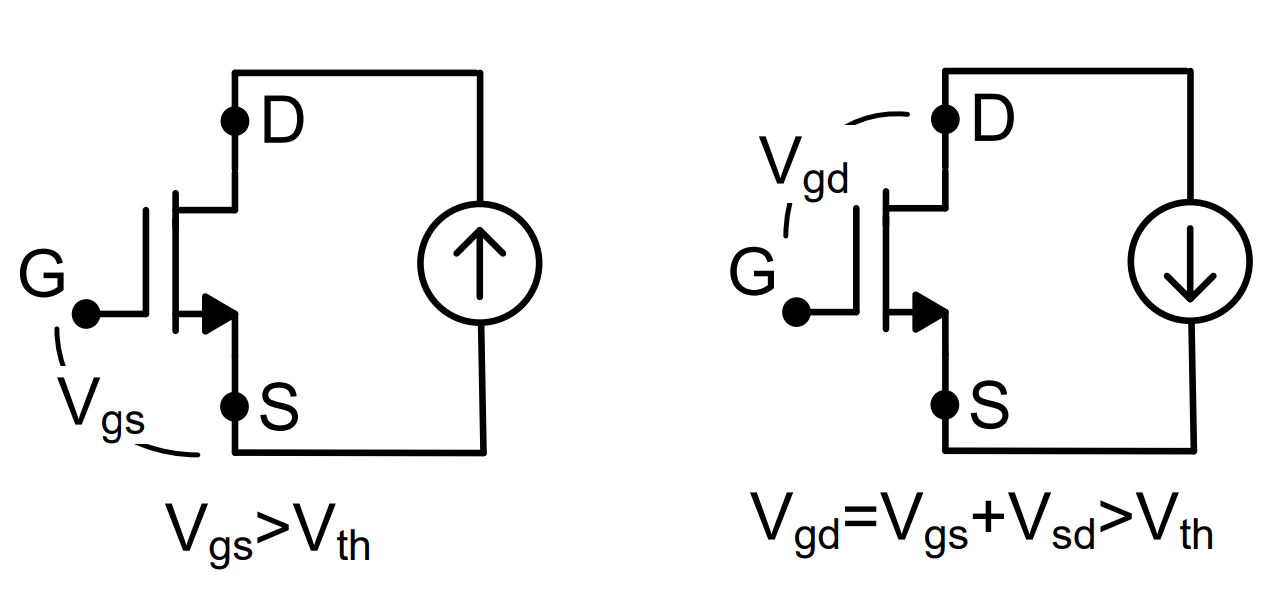
\includegraphics[width=0.4\textwidth]{gan_on_condition.png}
    \end{center}
    \caption{เงื่อนไขที่จะทำให้ทรานซิสเตอร์แกนนำกระแสในทิศทางไปข้างหน้า และย้อนกลับ}
    \label{gan_on_condition}
\end{figure}

ถ้าหากพิจารณาตัวอย่างที่เกิดขึ้นจริงในอินเวอร์เตอร์เพื่อให้เห็นภาพพจน์ชัดเจนขึ้นได้ดังนี้

\begin{figure}[h!]
    \begin{center}
        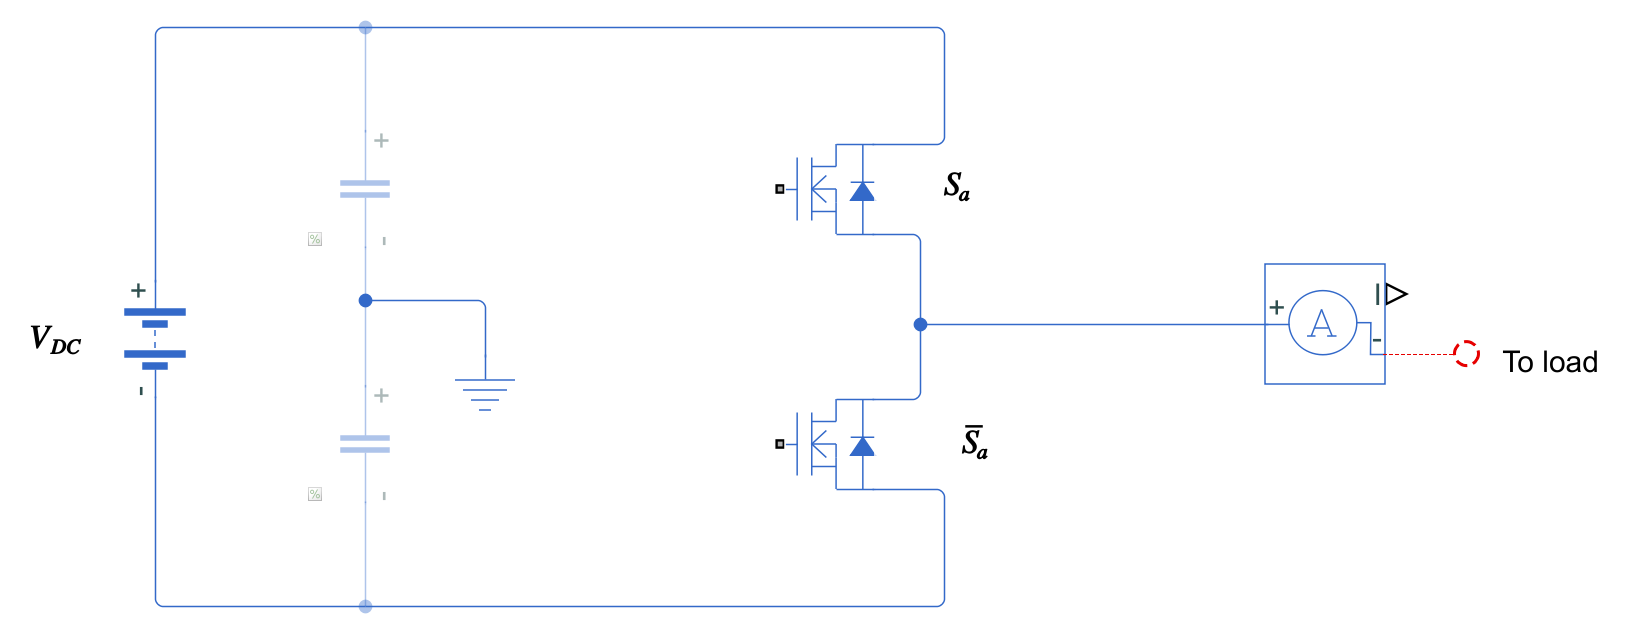
\includegraphics[width=0.7\textwidth]{first_third_inverter.png}
    \end{center}
    \caption{กรณีตัวอย่างการนำกระแสที่เกิดขึ้นจริงในอินเวอร์เตอร์}
\end{figure}

เรากำหนดให้สวิตช์ $S_a$ เป็นสวิตช์ที่เราสนใจ โดยถ้าหากเราขับนำสวิตช์ให้สวิตช์นำกระแส (On) นั่นคือ เราขับนำสัญญาณขา $V_{gs} > V_{th}$ แล้วถ้าหากโหลดที่ต่ออยู่กับขาซอร์สของสวิตช์ $S_a$ ดึงกระแสออกไปจากอินเวอร์เตอร์ นั่นคือ $I_a > 0$ จะทำให้ แรงดันตกคร่อมขาเดรนซอร์สของสวิตช์ $S_a$ เป็นค่าบวก นั่นคือ $V_{ds} > 0$ เนื่องจากสวิตช์ $S_a$ กำลังนำกระแสอยู่ ดังนั้นสวิตช์ $\bar{S_a}$ ไม่สามารถนำกระแสพร้อมๆ กับสวิตช์ $S_a$ ได้ เพราะจะลัดวงจร ดังนั้น กระแส $I_a$ ทั้งหมด ก็จะไหลผ่านสวิตช์ $S_a$ ทำให้กระแส $I_{ds} = I_a > 0$ เนื่องจากกระแส $I_{ds} > 0$ และ $V_{ds} > 0$ ดังนั้น สวิตช์นํากระแสในทิศทางไปข้างหน้า จุดทำงานที่กล่าวถึงข้างต้นจะแสดงในรูป \ref{inverter_q1}

\begin{figure}[h!]
    \begin{center}
        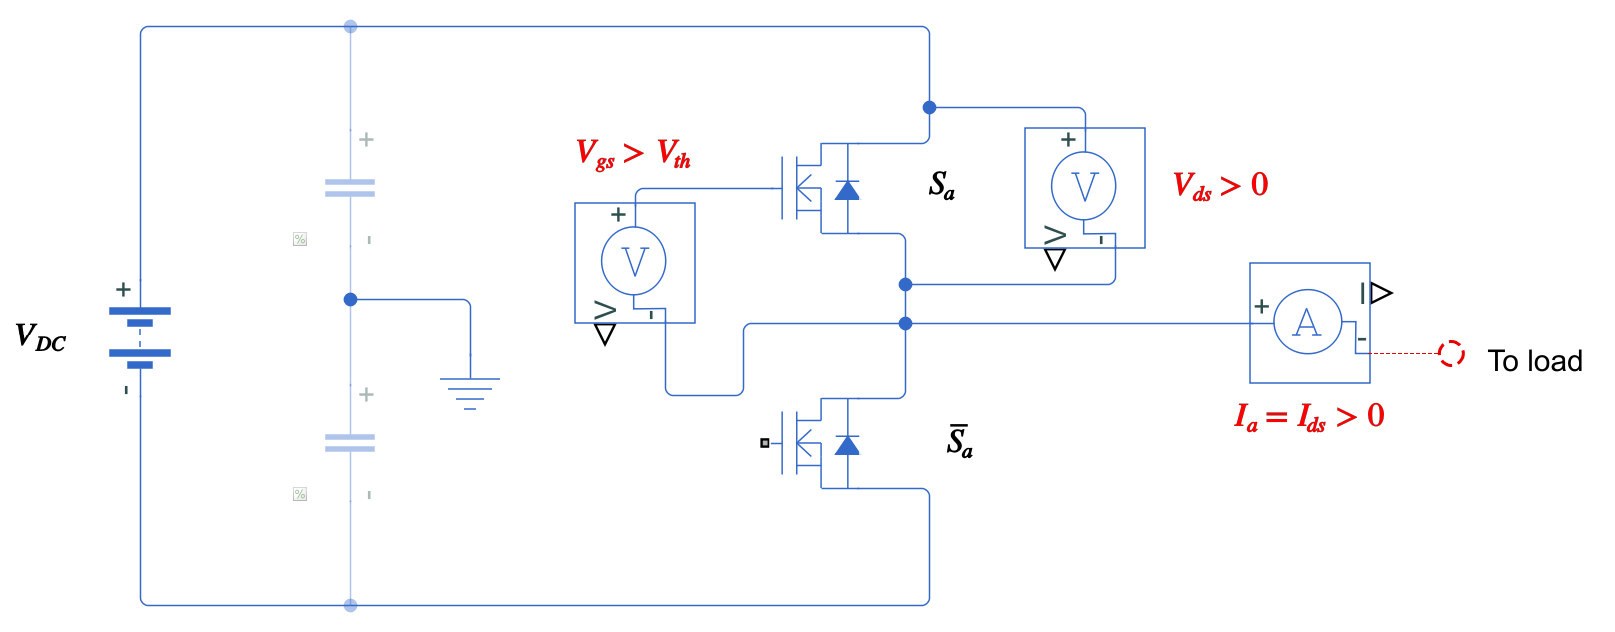
\includegraphics[width=0.7\textwidth]{inverter_q1.png}
    \end{center}
    \caption{กรณีตัวอย่างการนำกระแสในทิศทางไปข้างหน้า: $V_{gs} > V_{th}$, $I_{ds} > 0$}
    \label{inverter_q1}
\end{figure}

ถ้าหากพิจารณากรณีถัดไปคือการขับนำสวิตช์ในลักษณะเดิมคือ การขับสัญญาณขา $V_{gs} > V_{th}$ แต่มีสิ่งที่เปลี่ยนไปคือ ทิศทางการไหลของกระแส นั่นคือ ถ้าหากโหลดมีการดึงกระแสเข้าอินเวอร์เตอร์ $I_a = I_{sd} >0$ จะทำให้ แรงดันตกคร่อมขาเดรนซอร์สของสวิตช์เป็นค่าลบ นั่นคือ $V_{ds} <0; V_{sd} > 0$ เนื่องจาก $V_{gd} = V_{gs} + V_{sd} =($ ค่าที่มากกว่า $V_{th})+$ ค่าที่เป็นบวก ดังนั้น $V_{gd} > V_{th}$ และ $I_{ds} < 0$ ทำให้สวิตช์นำกระแสย้อนกลับ

\begin{figure}[h!]
    \begin{center}
        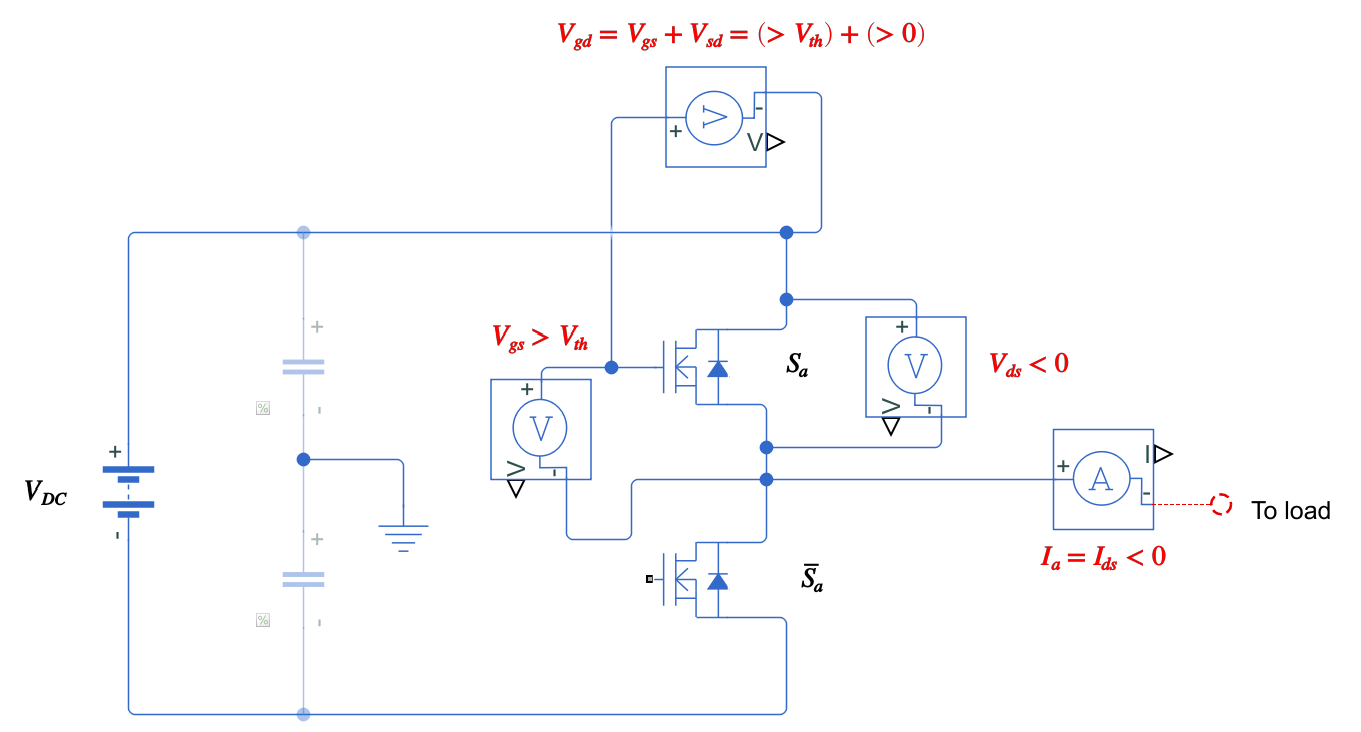
\includegraphics[width=0.7\textwidth]{inverter_q3.png}
    \end{center}
    \caption{กรณีตัวอย่างการนำกระแสในทิศทางย้อนกลับ: $V_{gd} > V_{th}$, $I_{ds} < 0$}
    \label{inverter_q1}
\end{figure}

เราจะสามารถเขียนความสัมพันธ์ของกระแสและแรงดันขณะนำกระแสไปข้างหน้าได้โดย

\begin{equation}
    V_{ds} = I_{ds}R_{ds(on)}
\end{equation}

เมื่อแรงดันที่ขาเกตเทียบกับซอร์สของทรานซิสเตอร์ มากกว่าค่าแรงดันขีดแบ่ง และแรงดันที่ขาเดรนเทียบซอร์สเป็นบวก จะทำให้แกนนำกระแสในจตุภาคที่หนึ่ง โดยที่เรานิยาม $R_{ds(on)}$ เป็นความต้านทานสมมูลของทรานซิสเตอร์ในขณะที่กำลังทำงานในจตุภาคที่หนึ่ง

และเราก็สามารถเขียนคามสัมพันธ์ของกระแสและแรงดันขณะนำกระแสย้อนกลับได้โดย

\begin{equation}
    V_{sd} = I_{sd}R_{sd(on)}
\end{equation}

ในการนำกระแสย้อนกลับ ข้อมูลต่างๆ จะเป็นทวิลักษณ์ของข้อมูลในขณะนำกระแสไปข้างหน้าเลยคือ เมื่อแรงดันที่ขาเกตเทียบกับเดรน มากกว่าค่าแรงดันขีดแบ่ง และแรงดันที่ขาซอร์สเทียบกับเดรนเป็นบวก จะทำให้ทรานซิสเตอร์นำกระแสในจตุภาคที่สาม

\begin{figure}[h]
    \begin{center}
        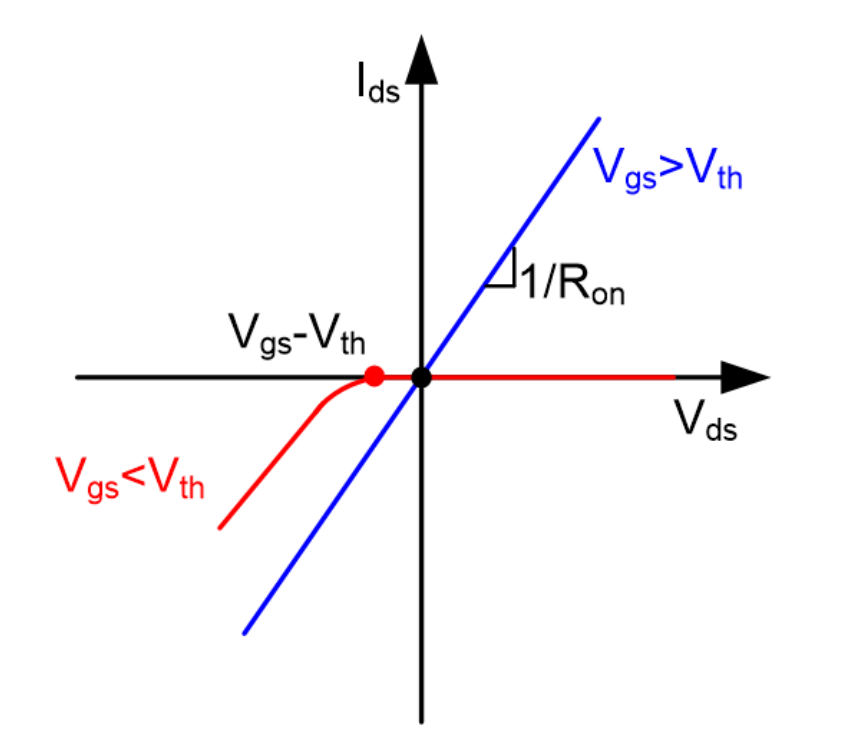
\includegraphics[width=0.4\textwidth]{gan_behavior.png}
    \end{center}
    \caption{พฤติกรรมการนำกระแสในจตุภาคที่หนึ่ง และจตุภาคที่สามของทรานซิสเตอร์แกน}
    \label{gan_behavior}
\end{figure}

จากรูปที่ \ref{gan_behavior} จะเห็นได้ว่า แรงดันตกคร่อมทรานซิสเตอร์ในจตุภาคที่สาม จะมากกว่าแรงดันตกคร่อมทรานซิสเตอร์ในจตุภาคที่หนึ่งที่ค่ากระแสเท่ากัน ซึ่งทำให้การนำกระแสในจตุภาคที่สามนั้นมีกำลังสูญเสียในขณะนำกระแสมากกว่าการนำกระแสในจตุภาคที่หนึ่ง

\subsubsection{การลดกำลังสูญเสียในการมอดูเลตแบบใช้สัญญาณพาหะ ด้วยการมอดูเลตแบบสองแขน}

จากที่ได้นำเสนอไปแล้วในส่วนของการมอดูเลตแบบ SPWM ว่า เป็นการมอดูเลตที่มีจำนวนครั้งในการสวิตช์มาก ซึ่งทำให้กำลังสูญเสียในขณะสวิตช์สูง แต่เรามีเทคนิคในการลดกำลังสูญเสียขขณะสวิตช์ในการมอดูเลตแบบ SPWM ด้วยการลดจำนวนครั้งในการสวิตช์คือ การมอดูเลตแบบสองแขน

แขนของการมอดูเลต คือ คู่ของทรานซิสเตอร์ที่ใช้ในการสร้างแรงดันออกที่ขั้วของอินเวอร์เตอร์ จะประกอบไปด้วยทรานซิสเตอร์ตัวบน ซึ่งเป็นทรานซิสเตอร์ที่ต่ออยู่กับบัสแรงดันไฟตรงที่ขั้วบวก และทรานซิสเตอร์ตัวล่าง ซึ่งเป็นทรานซิสเตอร์ที่ต่ออยู่กับบัสแรงดันไฟตรงที่ขั้วลบ จากทอพอโลยีของอินเวอร์เตอร์ที่เราเลือกใช้ในโครงงานฉบับนี้ ซึ่งแสดงไว้ ณ รูปที่ \ref{3phaseinv} จะเห็นได้ว่า จะมีแขนของการมอดูเลตทั้งหมดสามแขน

จากการพิจารณาจะเห็นได้ว่า หากเราต้องการสร้างแรงดันรูปไซน์ที่ขั้วของอินเวอร์เตอร์ เราจำเป็นต้องสวิตช์ทั้งสามแขนไปพร้อมๆ กัน แต่ถ้าหากเราพิจารณาความจริงที่ว่า แรงดันที่สร้างกระแสของมอเตอร์ที่ต่อแบบสามเฟสสามสาย เป็นแรงดันระหว่างสาย คือ

\begin{eqnarray}
    v_{ab} &=& v_{a0} - v_{b0} \\
    v_{bc} &=& v_{b0} - v_{c0} \\
    v_{ca} &=& v_{c0} - v_{a0}
\end{eqnarray}

และถ้าหากเราเพิ่มแรงดันลำดับศูนย์ (Zero Sequence Offset) ให้กับแรงดันเฟสของอินเวอร์เตอร์

\begin{eqnarray}
    v_{a0}^* &=& v_{a0} + v_{N0} \\
    v_{b0}^* &=& v_{b0} + v_{N0} \\
    v_{c0}^* &=& v_{c0} + v_{N0}
\end{eqnarray}

แรงดันระหว่างสายของมอเตอร์จะมีค่าเท่าเดิม นั่นคือ

\begin{eqnarray}
    v_{ab}^* &=& v_{a0}^* - v_{b0}^* = v_{a0} + v_{N0} - (v_{b0} + v_{N0}) = v_{ab} \\
    v_{bc}^* &=& v_{b0}^* - v_{c0}^* = v_{b0} + v_{N0} - (v_{c0} + v_{N0}) = v_{bc} \\
    v_{ca}^* &=& v_{c0}^* - v_{a0}^* = v_{c0} + v_{N0} - (v_{a0} + v_{N0}) = v_{ca}
\end{eqnarray}

ดังนั้น เราสามารถเลือกแรงดันลำดับศูนย์ที่จะเพิ่มให้กับแรงดันเฟสคำสั่งของอินเวอร์เตอร์ โดยมีเป้าหมายคือ ทำให้แรงดันคำสั่งในเฟสใดเฟสหนึ่งของอินเวอร์เตอร์ มีค่าเท่ากับแรงดันบวก หรือลบของบัสแรงดันกระแสตรง เพื่อที่จะทำให้แขนของการมอดูเลตแขนนั้น ปิด หรือ เปิดตลอดเวลา นั่นคือ

\begin{equation}
    V_{N0} = \begin{cases}
        \frac{V_{DC}}{2}-max(v_{a0},v_{b0},v_{c0}); \text{ทรานซิสเตอร์ตัวบน on ตลอด} \\
        \frac{-V_{DC}}{2}-min(v_{a0},v_{b0},v_{c0}); \text{ทรานซิสเตอร์ตัวล่าง on ตลอด}
    \end{cases}
\end{equation}

\subsubsection{การเพิ่มประสิทธิภาพให้กับการมอดูเลตแบบสองแขนด้วยการติดตามการทำงานในจตุภาคที่ 1}

จากผลลัพธ์ที่ได้อภิปรายมาในส่วนที่แล้ว เราได้ทราบว่า เรามีอิสระในเลือกการมอดูเลตสองแขนได้สองประเภทคือ แบบทรานซิสเตอร์ตัวบน on ตลอด และทรานซิสเตอร์ตัวล่าง on ตลอด ดังนั้น เราจะใช้ข้อได้เปรียบนี้ ในการเลือกรูปแบบการมอดูเลตแบบสองแขนให้เกิดประสิทธิภาพสูงที่สุด นั่นคือ การหลีกเลี่ยงการทำงานในจตุภาคที่ 3 สำหรับทรานซิสเตอร์ตัวที่มีแรงดันมากที่สุด หรือน้อยที่สุดในขณะนั้น

\subsection{การเพิ่มประสิทธิภาพของแผ่นพื้นเก็บพลังานด้วยอัลกอริทึมการติดตามจุดทำงานที่ให้กำลังสูงสุด (Maximum Power Point Tracking Algorithm; MPPT)}
\subsubsection{ข้อมูลรายละเอียดและหลักการทำงานของแผ่นพื้นเก็บพลังงาน}
เริ่มแรกต้องเข้าใจหลักการทำงานของแผ่นพื้นเก็บพลังงานเพื่อทราบความสัมพันธ์ของกลไกและสมการต่างๆของระบบทางกลของแผ่นพื้นเก็บพลังงาน จากนั้นจึงสามารถแปลงเป็นวงจรสมมูลทางไฟฟ้าได้ต่อไป

แผ่นพื้นเก็บพลังงาน สามารถแปลงพลังงานจลน์จากการก้าวเดินของมนุษย์แปลงเป็นพลังงานไฟฟ้าจากเครื่องกำเนิดไฟฟ้าได้ หลักการทำงาน เริ่มจากการเหยียบของมนุษย์ลงบนแผ่นพื้นเก็บพลังงานทำให้เกิดการยุบตัวลงของแผ่นพื้น nut จะขยับขึ้นลงไปขับเกลียวนำ(lead screw) ซึ่งทำหน้าที่เปลี่ยนแนวการเคลื่อนที่เชิงเส้นไปยังการเคลื่อนที่เชิงหมุน ให้หมุนรอบแนวแกนตั้ง และ bevel gear ทำหน้าที่เปลี่ยนจากเคลื่อนที่เชิงหมุนแนวแกนตั้งจากเพลาเกลียวนำให้เปลี่ยนทิศทางการหมุนไป 90 องศา หมุนรอบแนวนอน เพื่อขับเครื่องกำเนิดไฟฟ้า ดังรูปที่ \ref{lead-screw_lx}

\begin{figure}[h!]
    \begin{center}
        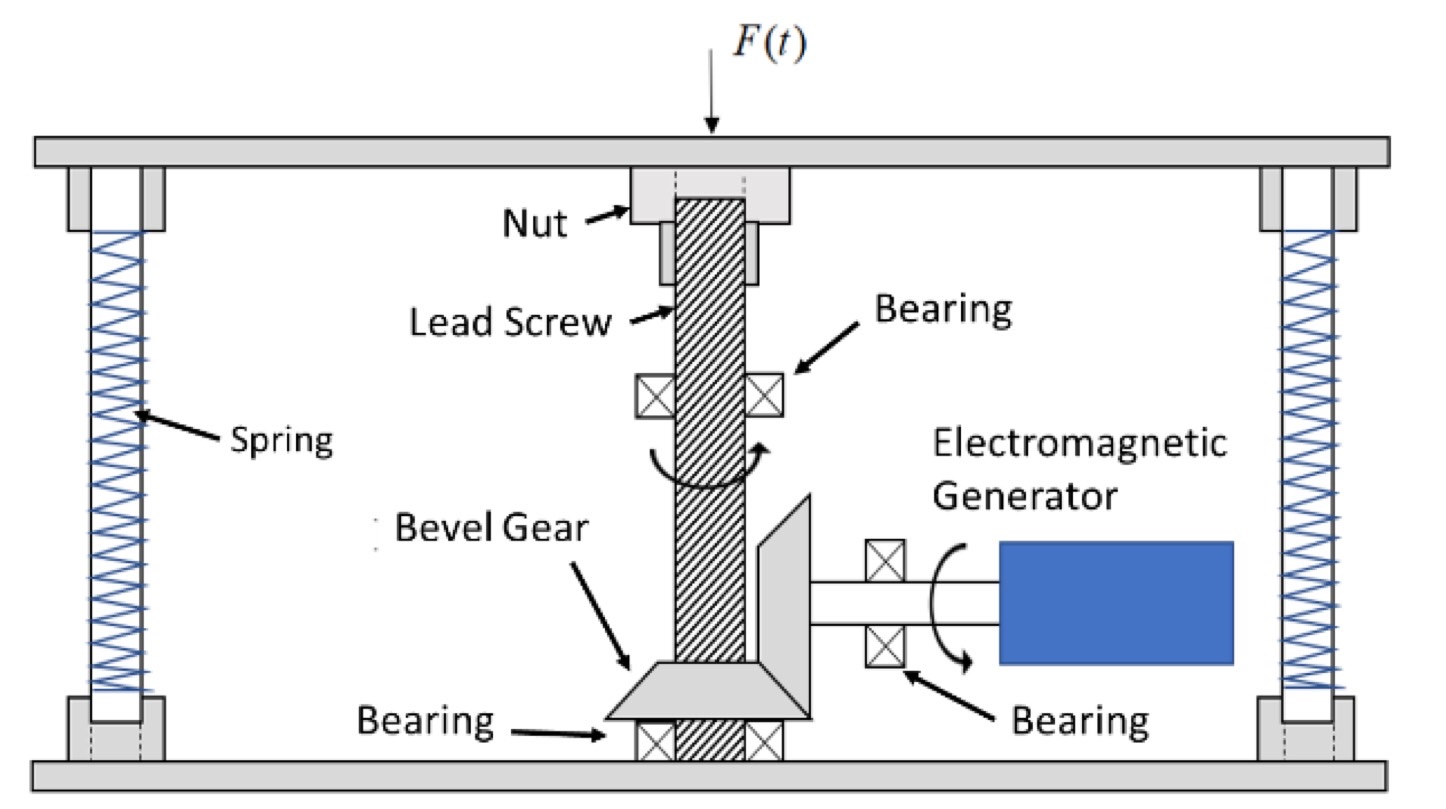
\includegraphics[width=0.5\textwidth]{lead-screw_lx.png}
    \end{center}
    \caption{กลไกเกลาตัวหนอน(lead screw) ภายใต้แผ่นเก็บพลังงาน}
    \label{lead-screw_lx}
\end{figure}

จากแผนภาพของวัตถุของระบบทางกล lead และ screw ดังรูปที่ 2 สมการต่างๆ ได้มาจาก การเลื่อนที่ของ nut และ การเคลื่อนที่เชิงหมุนของ lead screw และ โรเตอร์ของเครื่องกำเนิดไฟฟ้า ตามลำดับ ได้แก่
\newpage
\begin{equation}
    m\ddot{x} = F(t)-F_{a}-F_{s}
\end{equation}

\begin{equation}
    J_{1}\ddot{\theta}_{1} = \frac{2\pi J_{1}}{l}\ddot{x} = T_{a}-T_{B}
\end{equation}

\begin{equation}
    J_{G}\ddot{\theta}_{2} = \frac{2\pi J_{G}}{l}\ddot{x} = T_{B}-T_{G}
\end{equation}

\begin{figure}[h!]
    \begin{center}
        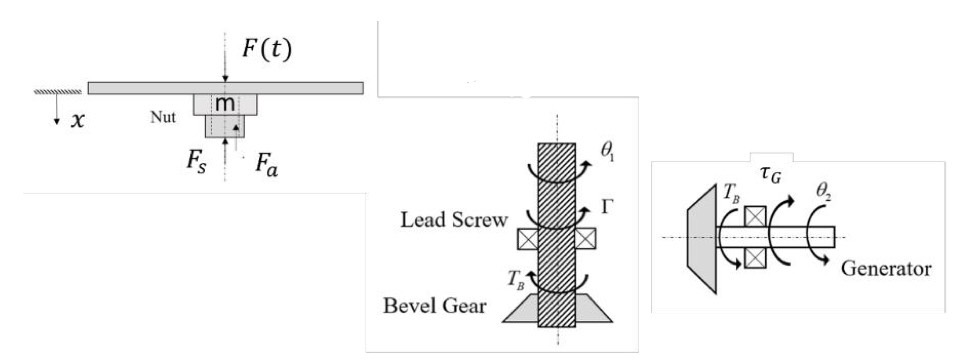
\includegraphics[width=0.7\textwidth]{free_body_lx.png}
    \end{center}
    \caption{แผนภาพของวัตถุของ lead screw}
    \label{free_body_lx}
\end{figure}

โดยที่

$m$ คือ มวลของแผ่นพื้น และ nut

$J_{1}$ คือ โมเมนต์ความเฉื่อยของ lead screw 

$J_{G}$ คือ โมเมนต์ความเฉื่อยของ bevel gear

$x$ คือ ระยะกระจัดของแผ่นพื้น และ nut

$l$ คือ ระยะห่างระหว่างเกลียวของ lead screw

$\theta_{1}$  คือ ตำแหน่งเชิงมุมของ lead screw 

$\theta_{2}$  คือ ตำแหน่งเชิงมุมของ bevel gear

$F(t)$  คือ แรงกดลงบนแผ่นพื้นที่เวลาใดๆ

$F_{s}$   คือ แรงสปริง

$F_{a}$   คือ แรงเสียดทานระหว่าง nut และ lead screw

$T_{B}$   คือ แรงบิดเสียดทานระหว่าง nut และ lead screw

$T_{G}$   คือ แรงบิดแม่เหล็กไฟฟ้า (Electromagnetic torque)

$T_{a}$   คือ แรงบิดส่งผ่านจาก nut และไปยัง lead screw ซึ่งเป็นสัดส่วนโดยตรงกับ $F_{a}$ ดังนี้

\begin{equation}
    T_{a} = aF_{a}
\end{equation}

ค่าคงที่ a = $\frac{l}{2\pi \eta_{tread} \eta_{thrust}}$ เมื่อ $\eta_{tread}$ คือ ประสิทธิภาพของตลับลูกปืนคลัตซ์ และ $\eta_{trhust}$ คือ ประสิทธิภาพของเกลียว

\subsubsection{Electrical analogy}
แบบจำลองทางไฟฟ้าที่ของระบบทางกลของแผ่นพื้นเก็บพลังงานสร้างโดยเริ่มจาก โดยใช้ electrical analogy เพื่อที่จะแปลงเป็นวงจรสมมูลทางไฟฟ้า

Analogy ของวงจรไฟฟ้าเป็นประโยชน์อย่างมากเมื่อทำการวิเคราะห์ระบบทางกล ปัญหาทางกลบางอย่างสามารถแก้ไขได้ง่ายขึ้นผ่านการเปรียบเทียบทางไฟฟ้า analogy ที่ใช้งานทั่วไปมีเป็นสิ่งที่สัมพันธ์กันของปริมาณทางกลและทางไฟฟ้า ดังแสดงในตารางที่ 1 

\begin{center} 
    ตารางที่ 1 แสดงความสัมพันธ์ของปริมาณทางกลและไฟฟ้า
    \end{center} 
\begin{figure}[h!]
    \begin{center}
        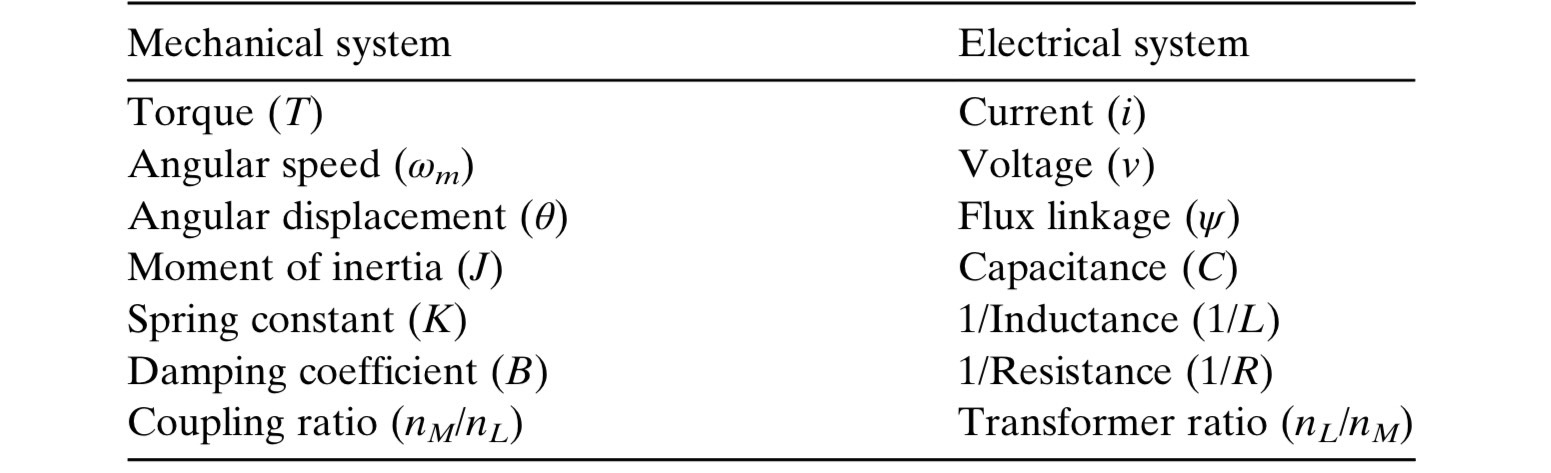
\includegraphics[width=0.7\textwidth]{analogy_lx.png}
    \end{center}
    \label{analogy_lx}
\end{figure}
เนื่องจากอัตราส่วนของเกียร์ของ gear train และ bevel gears ที่ใช้ในการส่งการเคลื่อนที่เชิงหมุนจาก lead screw ไป ยังโรเตอร์ของเครื่องกำเนิดไฟฟ้า มีอัตราส่วนเท่ากับ 1:1 จึงได้ความสัมพันธ์ 
\begin{equation}
    x = \frac{l\theta_{1}}{2\pi} = \frac{l\theta_{2}}{2\pi} 
\end{equation}
จากสมการที่ (18)-(20) ทำการเปลี่ยนแนวการเคลื่อนที่เชิงเส้นไปยังการเคลื่อนที่เชิงหมุน และใช้ความสัมพันธ์ของปริมาณทางกลและไฟฟ้าจากตารางที่ 1 
\begin{equation}
   \frac{aml}{2\pi}\ddot{\theta}_{1} + \frac{aDl}{2\pi}\dot{\theta}_{1} + \frac{akl}{2\pi}\theta_{1} + aF_{a} = aF_(t)
\end{equation}
\begin{equation}
    J_{1}\ddot{\theta}_{1} + T_{B} = aF_{a}
 \end{equation}
 \begin{equation}
    J_{G}\ddot{\theta}_{2} + T_{G} = T_{B}
 \end{equation}
 \begin{figure}[!htb]
    \begin{center}
        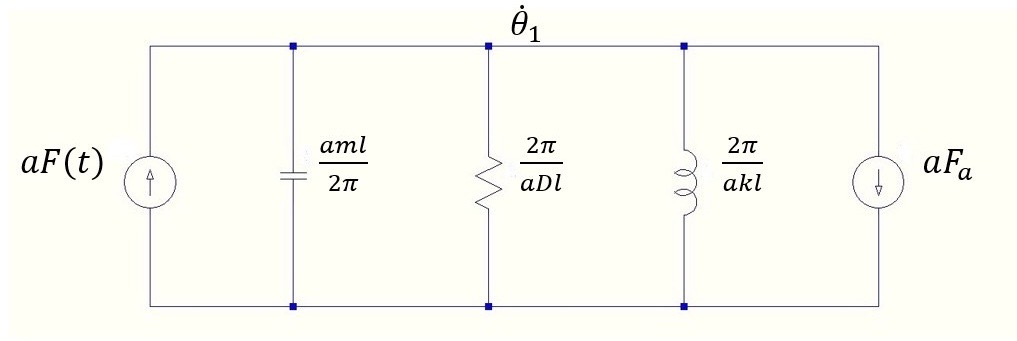
\includegraphics[width=0.7\textwidth]{cir1lx.jpeg}
    \end{center}
    \caption{วงจรไฟฟ้าของการเลื่อนที่ของ nut}
    \label{cir1lx}
\end{figure}
\begin{figure}[!htb]
    \begin{center}
        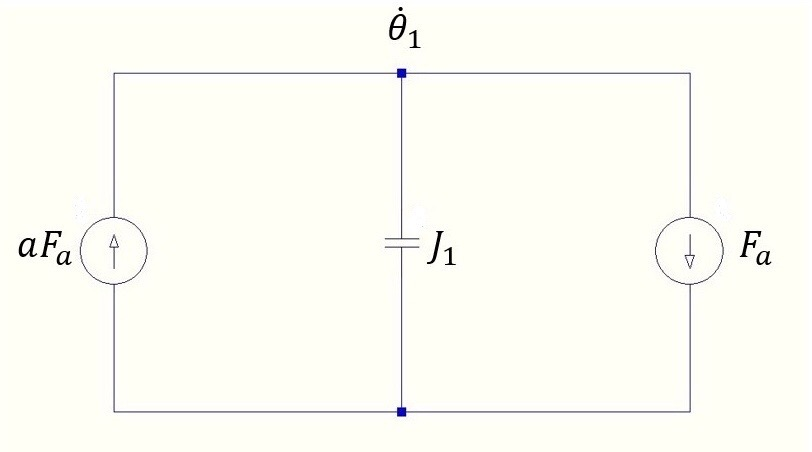
\includegraphics[width=0.5\textwidth]{cir2lx.jpg}
    \end{center}
    \caption{วงจรไฟฟ้าของการเคลื่อนที่เชิงหมุนของ lead screw }
    \label{cir2_lx}
\end{figure}
\begin{figure}[!htb]
    \begin{center}
        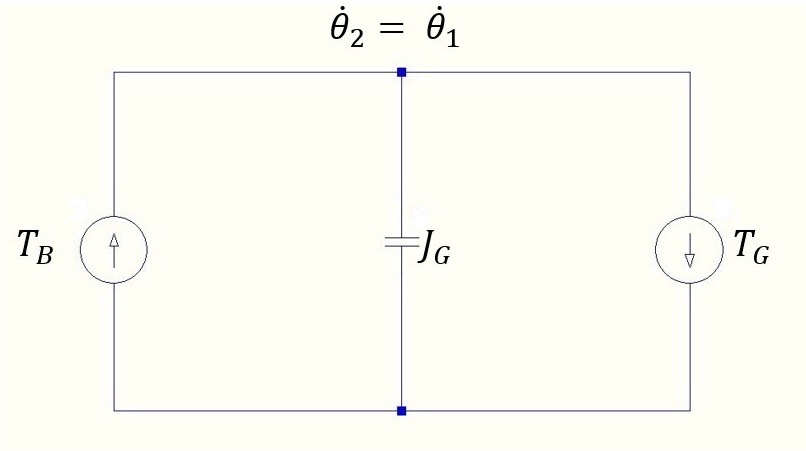
\includegraphics[width=0.5\textwidth]{cir3lx.jpg}
    \end{center}
    \caption{วงจรไฟฟ้าของโรเตอร์ของเครื่องกำเนิดไฟฟ้า}
    \label{cir3lx}
\end{figure}
จากรวมวงจรทั้งสามข้างบน จะได้ วงจรสมมูลทางไฟฟ้าระบบทางกลของแผ่นพื้นเก็บพลังงาน
\begin{figure}[!htb]
    \begin{center}
        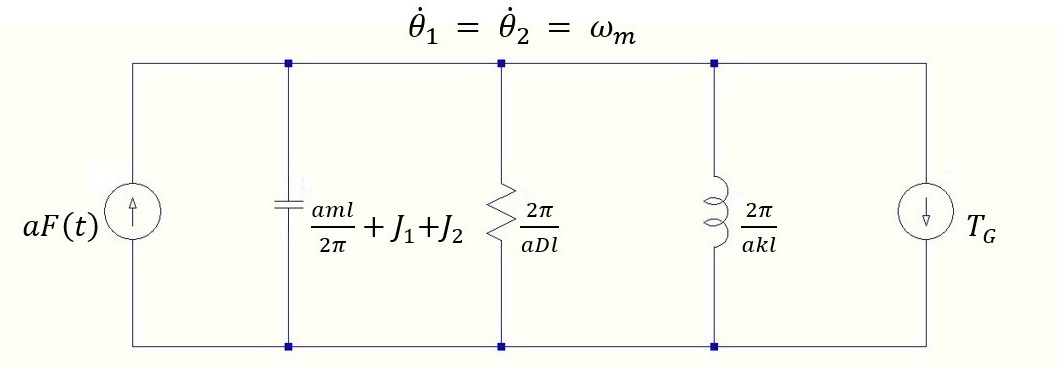
\includegraphics[width=0.7\textwidth]{cir4lx.jpg}
    \end{center}
    \caption{วงจรสมมูลทางไฟฟ้าของระบบทางกลของแผ่นพื้นเก็บพลังงาน}
    \label{cir4lx}
\end{figure}



\newpage
\section{ผลลัพธ์จากการดำเนินการเบื้องต้น}
\begin{figure}[!htb]
    \centering
    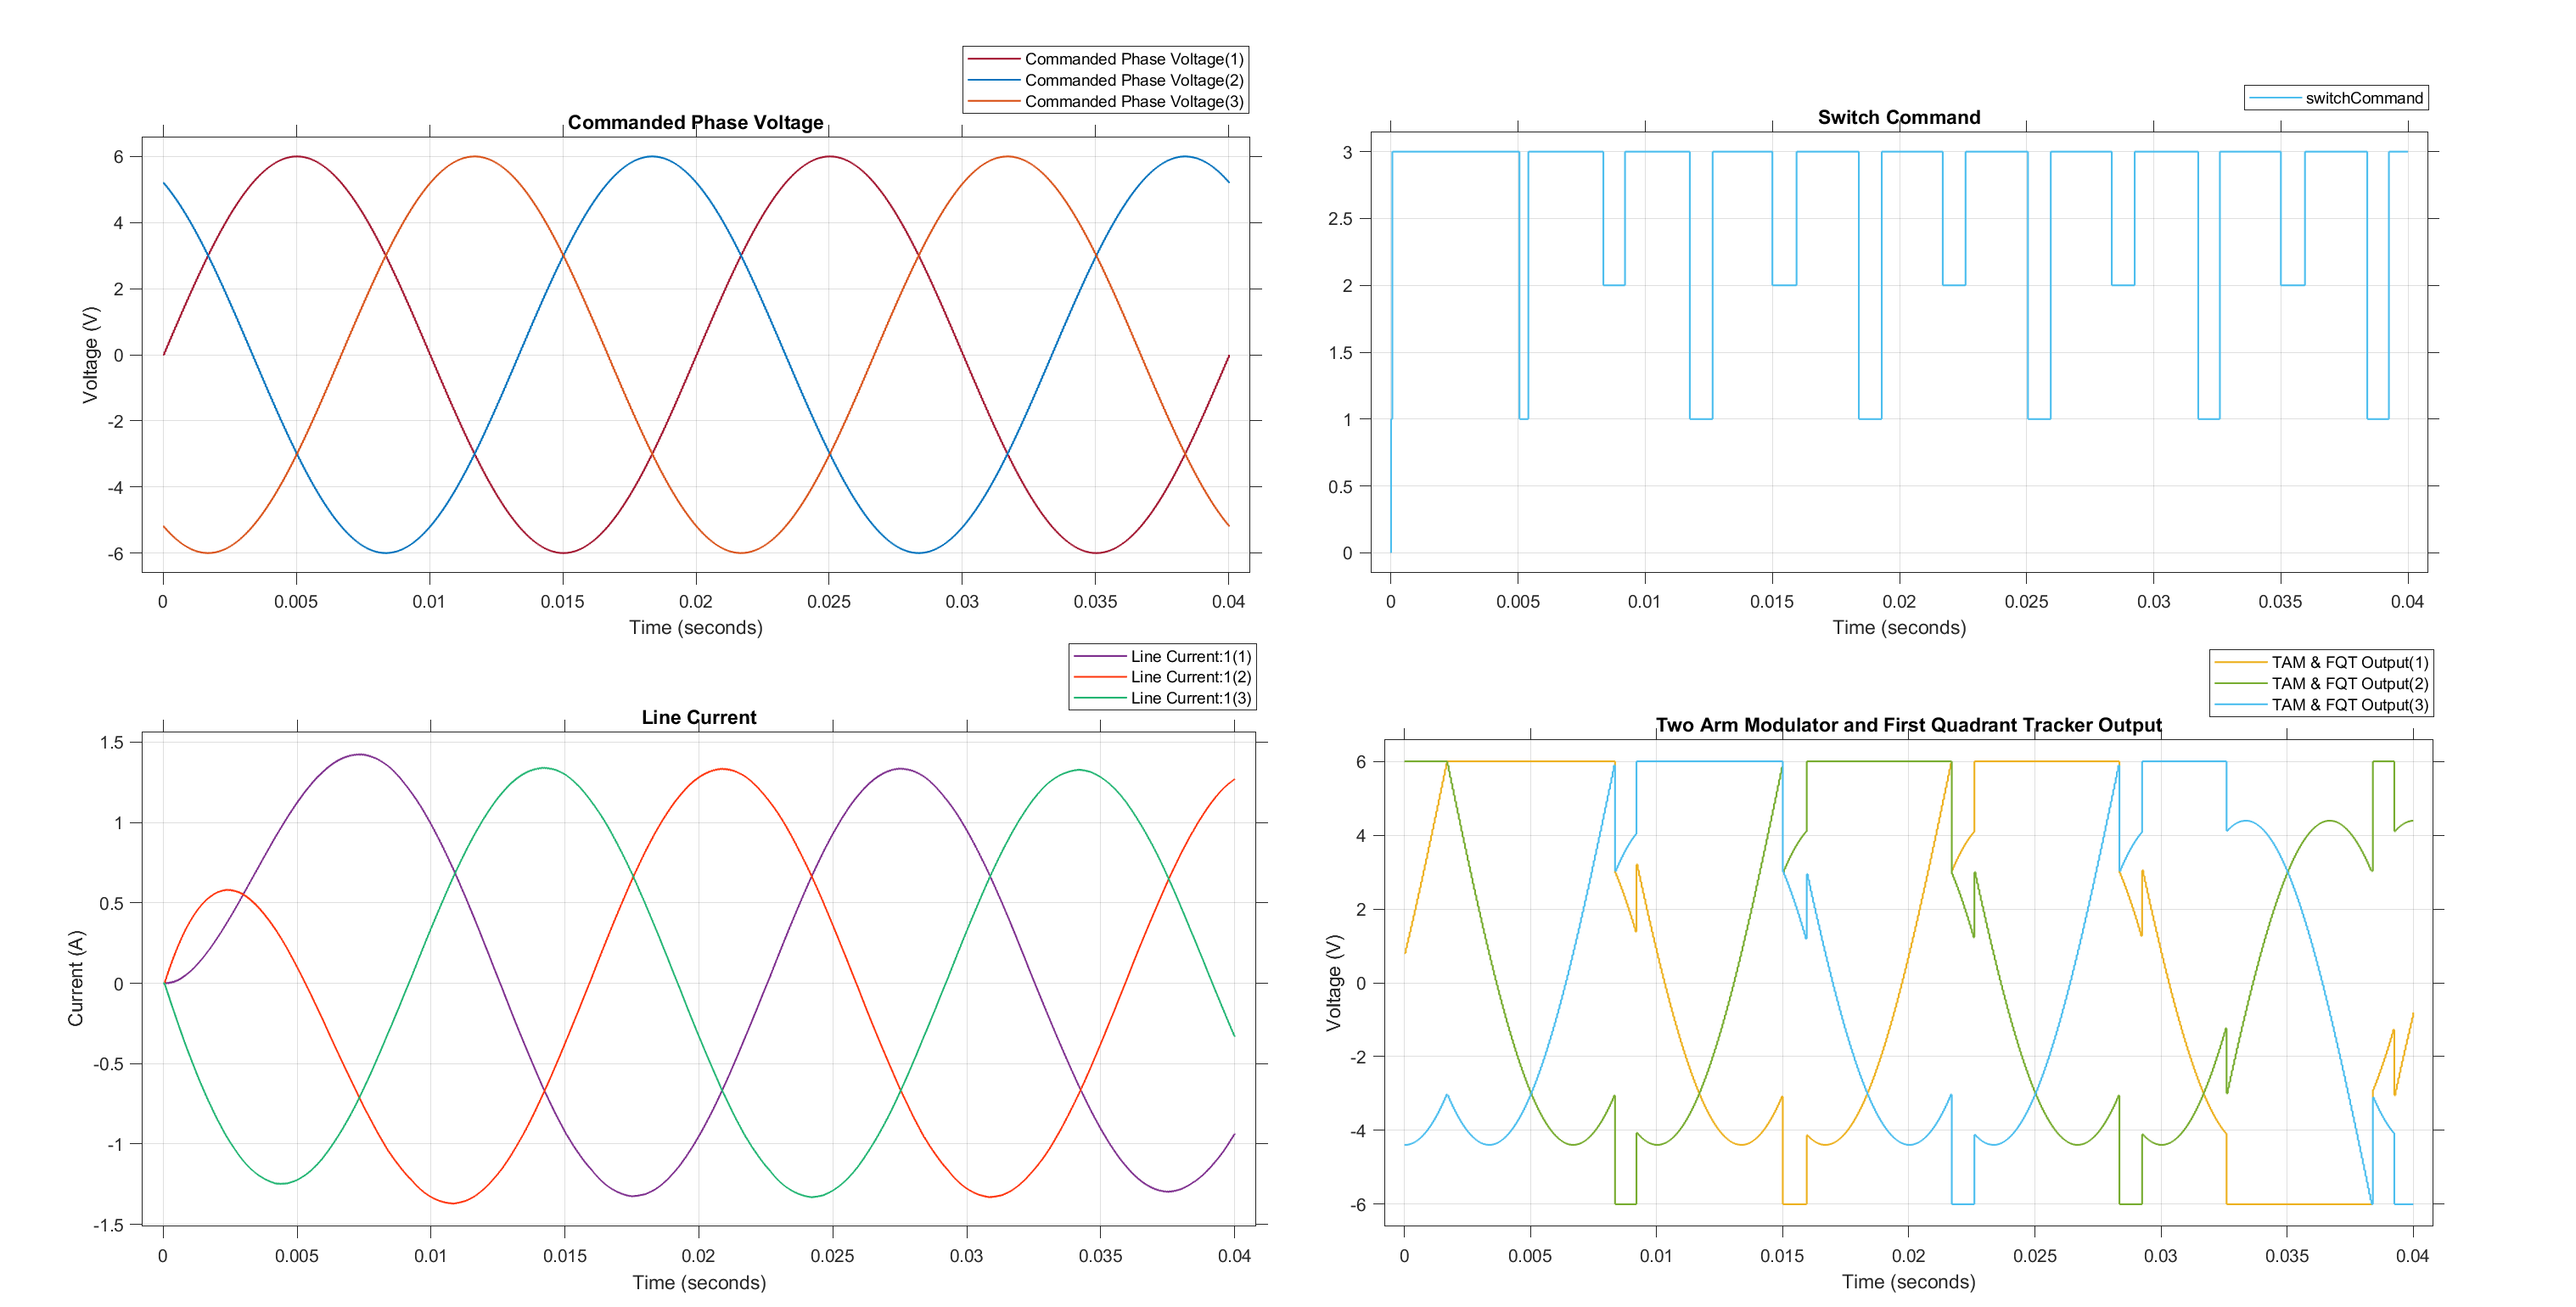
\includegraphics[width=\textwidth]{VSI_6V_50Hz_3Ohm_10mH.eps}
    \caption{50Hz}

\end{figure}

% ในส่วนนี้ให้นิสิตได้ผลลัพธ์หรือผลสำเร็จอะไรมาบ้าง จากการดำเนินโครงงานตามแผนงานที่นิสิตได้นำเสนอไว้ตามแผนภูมิแกนต์ (Gantt chart) โดยปกติแล้วเมื่อเสร็จสิ้นขั้นตอนแต่ละขั้นตามแผนภูมิแกนต์ นิสิตควรจะได้ผลลัพธ์อย่างน้อยหนึ่งอย่างออกมา เช่นในขั้นตอนการศึกษาทฤษฎีที่เกี่ยวข้อง นิสิตน่าจะได้ข้อสรุปวรรณกรรม หรือข้อกำหนด (Specification) ออกมา หรือในขั้นตอนการออกแบบ นิสิตอาจได้แผนภาพบล็อก หรือร่างวงจรเบื้องต้นออกมาเป็นต้น สำหรับแต่ละขั้นตอน นิสิตควรอธิบายว่าได้ผลลัพธ์นั้นมาได้อย่างไร ถูกต้องตามหลักการทางวิศวกรรมหรือไม่ มีตัวเลือก (Choice) อะไรบ้างในขั้นตอนต่างๆ อาจมีผลการทดลอง ผลการจำลองเบื้องต้น เช่น กราฟ ตาราง เป็นต้น และการวิเคราะห์ อภิปรายผลมาประกอบ เพื่อโน้มน้าวให้ผู้อ่านเชื่อว่าหัวข้อโครงงานที่นำเสนอนี้มีโอกาสประสบผลสำเร็จ ในหัวข้อนี้ นิสิตอาจจะแบ่งเป็นหัวข้อย่อย (ตามผลการทดลอง หรืออย่างไรก็แล้วแต่) ตามความเหมาะสม


% นิสิตควรเลือกนำเสนอผลลัพธ์เบื้องต้นที่สำคัญ ซึ่งต้องไม่ใช่สิ่งที่ง่าย (Trivial) เกินไป เช่น การใส่ผลการทดลองการหัดใช้โปรแกรม MATLAB การใส่วิธีการเขียนโค้ดภาษา Python ภาษา Java หรือภาษาอื่นๆ ในระดับเบื้องต้น หรือการทดลองใช้บอร์ดทดลองซึ่งไม่เกี่ยวกับโครงงานที่ทำ ตัวอย่างผลลัพธ์ที่นิสิตควรนำเสนอ เช่น


% หัวข้อโครงงานเป็นการใช้หลักการควบคุมเชิงทำนายแบบจำลอง ในการควบคุมกระบวนการ XX ในหัวข้อนี้ นิสิตอาจจะนำเสนอแบบจำลองทางคณิตศาสตร์ของระบบ YY พร้อมคำอธิบาย โดยมีผลการจำลองเบื้องต้นของการใช้ตัวควบคุมกับระบบ YY


% หัวข้อโครงงานเป็นการแยกแยะรูปภาพออกเป็นหลายคลาส (Class) โดยวิธี XX โค้ดด้วยภาษา YY ในหัวข้อนี้ นิสิตอาจะนำเสนอลักษณะเด่นของภาษา YY เปรียบเทียบกับภาษาอื่นๆ และโค้ดที่ได้เขียนขึ้นในเบื้องต้นเพื่อการวิเคราะห์รูปภาพ (Image Processing) หากโค้ดที่เขียนมีการเรียกใช้ไลบราลี (Library) คล้ายคลึงกับงานอื่นๆ นิสิตควรอธิบายได้ว่า ความซับซ้อนของปัญหาที่จะทำนั้นแตกต่างอย่างไร และนิสิตต้องทำอะไรเพิ่มเติมด้วยตนเองบ้าง


% หัวข้อโครงงานเป็นการสร้างต้นแบบอุปกรณ์ ระบบ หรือเครื่องมือหนึ่งๆ เช่น หุ่นยนต์ ระบบฝังตัวเพื่อการประยุกต์ XX ในหัวข้อนี้ นิสิตอาจะนำเสนอแบบร่างหรือแผนภาพบล็อกที่สมบูรณ์ของอุปกรณ์พร้อมระบุข้อกำหนดว่า อุปกรณ์จะประกอบไปด้วยชิ้นส่วนใด หรือบอร์ดใดบ้าง แต่ละชิ้นส่วน (เช่น มอเตอร์) หรือบอร์ด จะใช้รุ่นใด ความสามารถเป็นอย่างไร พร้อมทั้งอธิบายได้ว่า ทำไมเลือกข้อกำหนดอย่างนั้น หรือบอร์ดนั้นๆ รวมถึงซอฟต์แวร์ที่ใช้ในการพัฒนาโปรแกรมควบคุม นอกจากนี้ควรแสดงแผนภาพเชื่อมโยงของชิ้นส่วนแต่ละชิ้นว่าประกอบเป็นอุปกรณ์ต้นแบบที่สมบูรณ์ได้อย่างไร อาจนำเสนอผลการจำลองสมรรถภาพ (Efficiency) เบื้องต้น ภายใต้เงื่อนไขที่กำหนดไว้ด้วยก็ได้


% ขอให้นิสิตใส่ใจกับความชัดเจนของข้อมูล กราฟทุกกราฟ ตารางทุกตาราง เมื่อพิมพ์รายงานลงบนกระดาษขาวดำแล้ว ต้องสามารถอ่านได้ แยกเส้นกราฟได้ อ่านคำอธิบายกราฟ (Legend) ได้ มีคำกำกับแกนและคำอธิบายรูปกราฟชัดเจน รูปกราฟควรใช้เป็นแบบเวกเตอร์ (Vector Graphic) เนื่องจากรูปแบบเวกเตอร์จะสามารถยืดขยายได้ ไม่เหมือนกับรูปไบนารี่ (Binary) ที่เก็บรายละเอียดแบบพิกเซล (Pixel) ซึ่งจะเสียความละเอียด (Resolution) ไปเมื่อขยายรูปให้ใหญ่ขึ้น ถ้าใช้โปรแกรม MATLAB ในการวาดกราฟ ไม่ควรบันทึกรูปเป็นไฟล์ JPG แล้วนำมาวางในรายงานบนโปรแกรม Microsoft Word เพราะจะได้รูปที่ไม่คมชัด ให้นิสิตใช้คำสั่ง Copy Figure ซึ่งอยู่ในเมนู Edit ของหน้าต่างรูปกราฟของโปรแกรม MATLAB แล้วจึงนำมาวางในรายงาน จะได้รูปที่ชัดเจนกว่า หากข้อมูลเป็นตาราง ในส่วนของคำอธิบายตารางต้องบอกให้ชัดเจนว่า ตัวเลขในตารางคืออะไร หน่วยอะไร ควรมีการเน้นตัวเลขในตารางเพื่อให้ผู้อ่านสังเกตความแตกต่างได้โดยง่าย

\section{บทสรุป}
\subsection{สรุปผลการดำเนินการ}
% ในส่วนนี้ ให้นิสิตสรุปว่าได้ดำเนินการอะไรมาแล้วบ้างตั้งแต่ต้นจนถึงปัจจุบัน และจะดำเนินการอะไรต่อไป เพื่อให้โครงงานนี้เสร็จสมบูรณ์ ได้ผลลัพธ์ครบถ้วนตามวัตถุประสงค์และขอบเขตที่ได้กำหนดไว้

\subsection{แผนการดำเนินงาน}
ในรายงานฉบับนี้ มีแผนการดำเนินงานแยกเป็นของผู้จัดทำแต่ละคน คือ ของนายณัฐพล กาบแก้ว ซึ่งมีแผนการดำเนินงานดังแสดงในรูปที่ ~\ref{fig:ganttjob} และของนายสันติ ว่องประเสริฐ ซึ่งมีแผนการดำเนินงานดังแสดงในรูปที่ x
\begin{figure}[h]
    \noindent\resizebox{0.9\textwidth}{!}{
        \begin{tikzpicture}
            \begin{ganttchart}[
                    hgrid,
                    vgrid,
                    x unit = 1.2cm,
                    y unit title= 0.8cm,
                    time slot format=isodate-yearmonth,
                    time slot unit=month
                ]{2015-08}{2016-05}
                \gantttitlecalendar{year, month=shortname}\\
                \ganttbar[
                    bar/.append style={fill=black}
                ]{Literature Review}{2015-08}{2015-10} \\
                \ganttbar[
                    bar/.append style={fill=black}
                ]{Exploration on given data}{2015-10}{2015-11}\\
                \ganttbar[
                    bar/.append style={fill=black},
                    progress=100]{Frequency domain analysis}{2015-11}{2015-12}\\
                \ganttbar{Classification on generated data}{2016-01}{2016-02}\\
                \ganttbar{Classification on real data}{2016-02}{2016-03}\\
                \ganttbar{Improvement on the classification method}{2016-03}{2016-04}\\
                \ganttbar{Report summary}{2016-04}{2016-05}
            \end{ganttchart}
        \end{tikzpicture}
    }
    \caption{\label{fig:ganttjob} Gantt chart ของนายณัฐพล กาบแก้ว}
\end{figure}

\subsection{ปัญหา อุปสรรค และแนวทางแก้ไข (ถ้ามี)}
% ในหัวข้อนี้ ให้นิสิตกล่าวถึง ปัญหาและอุปสรรคที่ได้พบระหว่างการดำเนินงานมาจนถึงปัจจุบัน และให้อธิบายว่านิสิตได้หลบเลี่ยงหรือแก้ไขปัญหาอย่างไรบ้าง เช่น ถ้าต้องมีการเปลี่ยนแปลงวิธีการ เงื่อนไข หรือผลลัพธ์ที่ตั้งใจไว้แต่แรก ควรบอกว่าด้วยเหตุผลอะไร และควรมีข้อมูลมารองรับการตัดสินใจนั้นๆ ด้วย

% \section{ตัวอย่างคำสั่งที่ใช้งานใน LaTeX}
% ในส่วนนี้จะแสดงตัวอย่างการใช้คำสั่ง LaTeX เบื้องต้น สำหรับ tutorial นั้นมีมากมายบน Internet ตัวอย่างเอกสารประกอบการใช้งาน LaTeX ภาษาไทยที่ดีอันหนึ่งคือจาก อ.ดร. ฑิตยา หวานวารี~\cite{cuthesis} เป็น template สำหรับวิทยานิพนธ์ของจุฬาลงกรณ์มหาวิทยาลัย แต่ได้อธิบายการใช้คำสั่งเบื้องต้นไว้โดยละเอียด

% \subsection{การใส่ตาราง}
% \begin{table}[ht]
%     \centering
%     \caption{ตัวอย่างตาราง}
%     \vspace{3mm}
%     \begin{tabular}{|l|c|c|r|} \hline
%         Item                     & Font     & Font Type & Font Size \\ \hline
%         Title                    & Garamond & Bold      & 20        \\
%         Author names             & Garamond & Bold      & 12        \\
%         Author affiliation/email & Garamond & Regular   & 11        \\
%         Abstract/Keywords        & Garamond & Regular   & 11        \\
%         Level 1 headings         & Garamond & Bold      & 12        \\
%         Level 2 headings         & Garamond & Bold      & 11        \\
%         Level 3 headings         & Garamond & Regular   & 11        \\
%         Figure/table captions    & Garamond & Regular   & 11        \\
%         Main text/References     & Garamond & Regular   & 11        \\ \hline
%     \end{tabular}
% \end{table}

% \subsection{การใส่รูป}
% การใช้รูปในงานที่ compile ด้วย \XeLaTeX จะใช้รูป format .eps, .pdf, .jpg, .png เป็นต้น ขอให้ใช้ vector graphic เป็นหลัก สำหรับรูปผลการทดลองหรือการวาดแผนผังต่างๆ เนื่องจากรูปแบบเวคเตอร์จะสามารถยืดขยายได้ไม่เหมือนกับรูป binary ที่เก็บรายละเอียดแบบ pixel และจะมีการเสีย resolution ไปหากขยายรูป zoom ให้ใหญ่ขึ้น
% \begin{figure}[ht]
%     \begin{center}
%         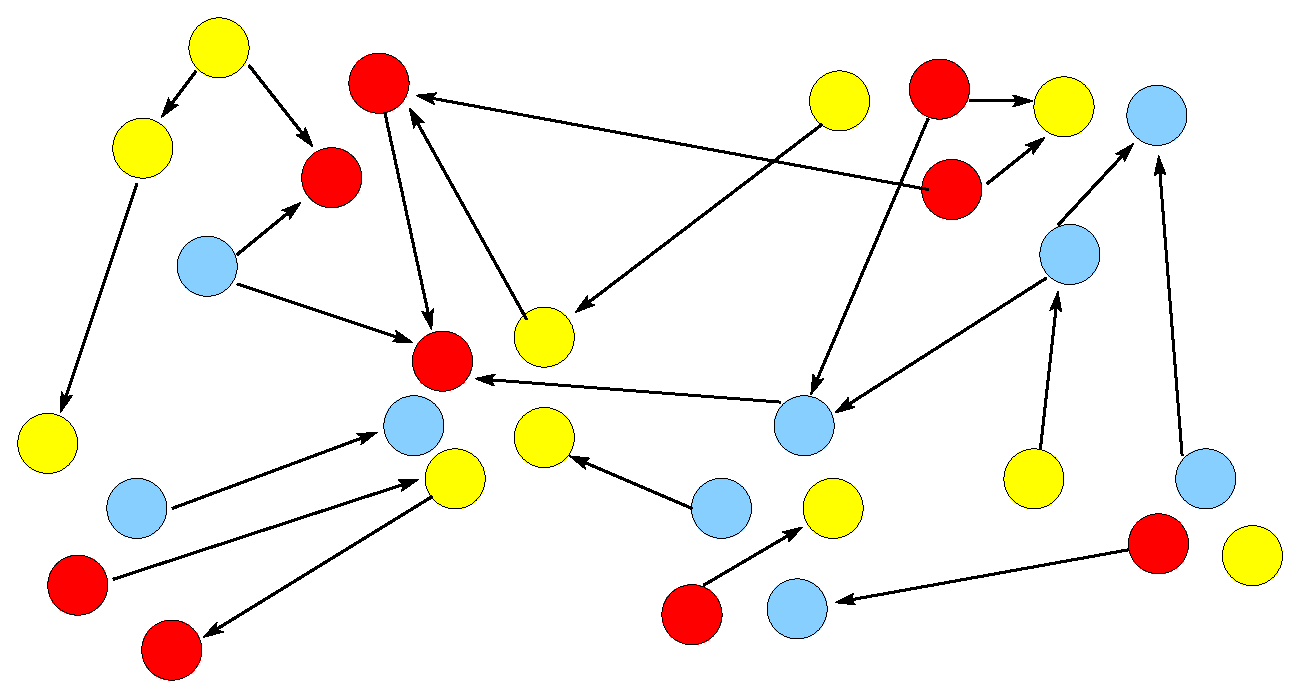
\includegraphics[width=0.7\linewidth]{gm.eps}
%         \caption{แบบจำลองเชิงกราฟ}
%     \end{center}
% \end{figure}

% \begin{figure}[h!]
%     \begin{center}
%         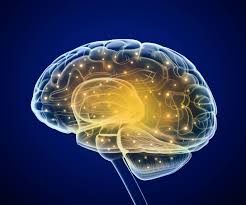
\includegraphics[width=0.5\linewidth]{brain.jpg}
%         \caption{สภาพการเชื่อมโยงของสมอง (ที่มา: Shutterstock.com รูปโดย: Alex Mit)}
%     \end{center}
% \end{figure}

% \begin{figure}
%     \centering
%     \subfigure[first caption]{ 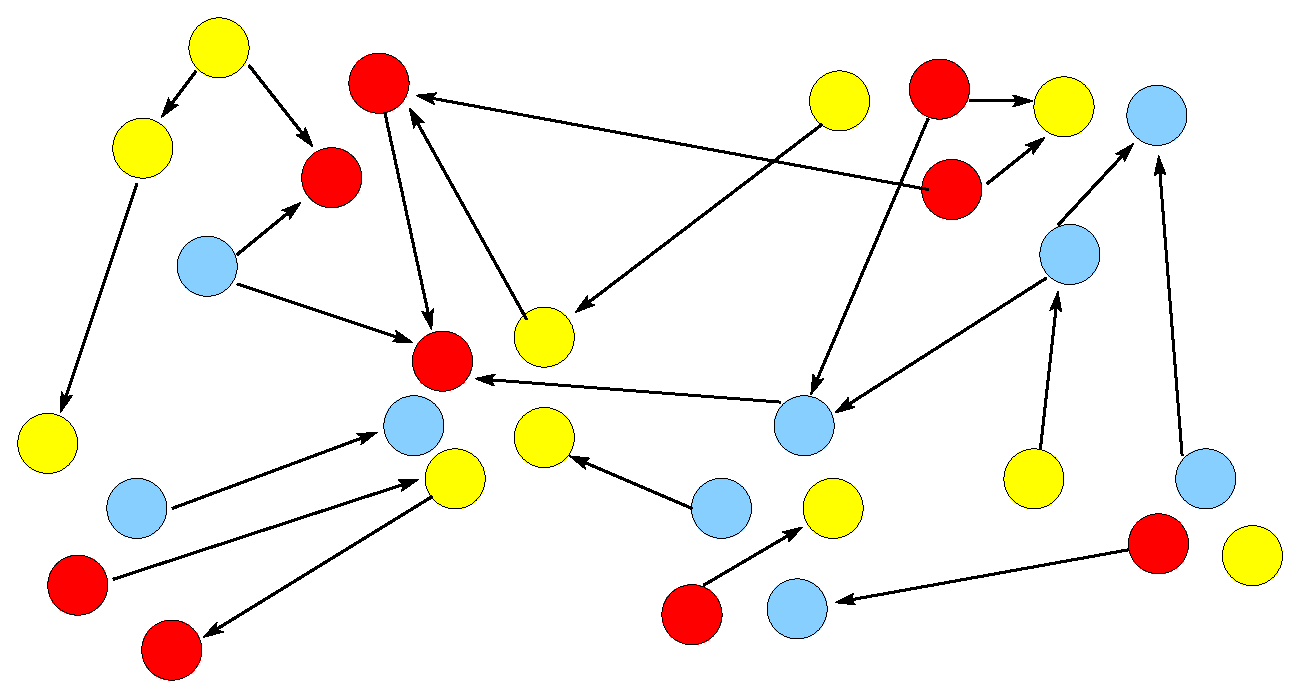
\includegraphics[width=0.45\linewidth]{gm.eps}  }
%     \subfigure[second caption]{ 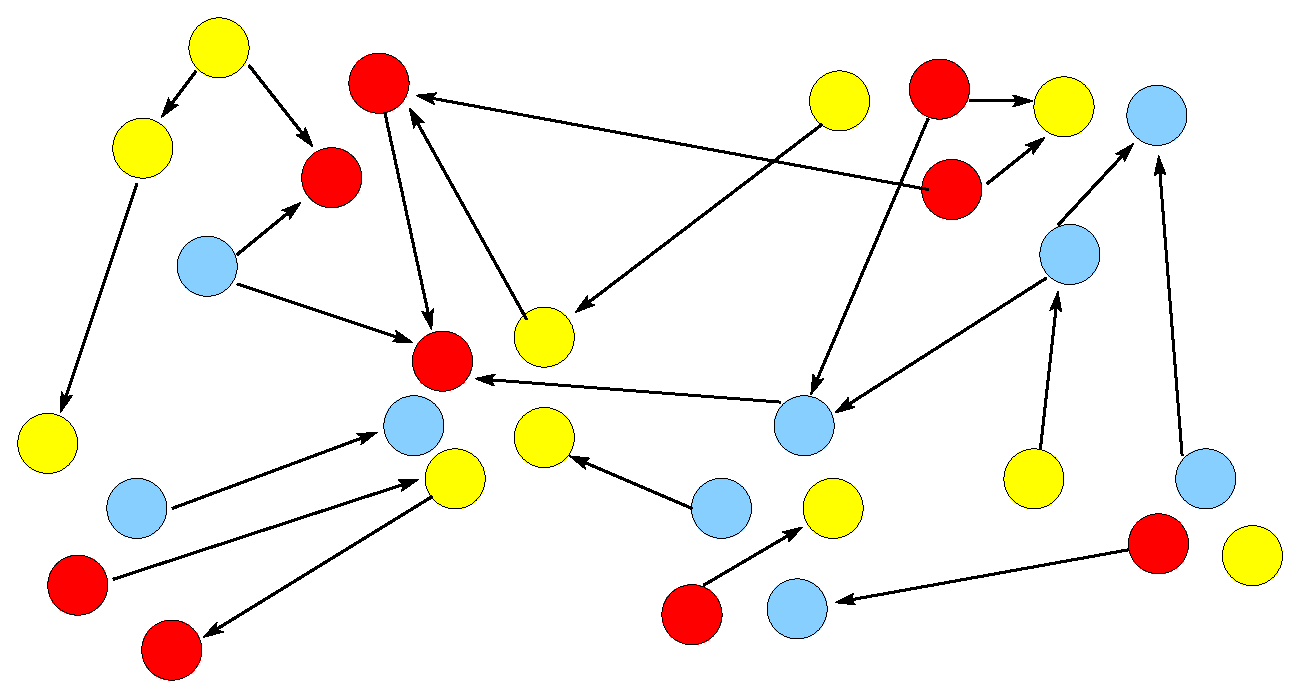
\includegraphics[width=0.45\linewidth]{gm.eps}  }
%     \caption{ตัวอย่างการใช้ subfigure}
% \end{figure}

% \subsection{การพิมพ์สมการ}
% กรณีพิมพ์สมการมีทั้งที่แทรกในบรรทัด เช่น $y=Cx$ หรือการแยกเป็นบรรทัดใหม่
% \begin{equation}
%     F(s) = \int_0^\infty e^{-st} f(t) dt
% \end{equation}

% การใช้ package 'align' จะสามารถเขียนสัญลักษณ์ต่างๆ ได้มากกว่า 1 บรรทัด มีได้หลายคอลัมน์ และสามารถจัดเรียงตำแหน่งได้ด้วย เช่น
% \begin{align}
%     x & = 2 \label{eq:x}       \\
%     y & = 3 \label{eq:y}       \\
%     z & = x \times y \nonumber \\
%       & = p \label{eq:results}
% \end{align}
% การไม่ใส่หมายเลขสมการ สามารถใช้คำสั่ง \texttt{\nonumber} หรือ \texttt{notag} ได้ โดยปกติแล้วหากไม่ใส่อะไรเลย สมการทุกสมการจะมีหมายเลขกำกับเสมอ หลักการใส่เลขสมการคือ จะใส่เลขสมการก็ต่อเมื่อสมการนั้นจะถูกอ้างถึงในภายหลัง ดังนั้นการอ้างอึง (cross reference) สามารถทำได้โดยใช้คำสั่ง \texttt{ref} หรือ \texttt{eqref} กับ \texttt{label} ตัวอย่างเช่น สมการ~\eqref{eq:x} กล่าวไว้ว่า $x=2$

% package 'eqnarray' ก็จะเป็นอีก environment หนึ่งที่ใช้เรียงสมการออกเป็น array

% \begin{eqnarray}
%     \dot{x} &=& Ax + Bu \\
%     y &=& Cx+Du
% \end{eqnarray}

% ถ้าหากมีสมการหลายบรรทัดและต้องการเรียงในแนว center ให้ใช้ package 'gather'
% \begin{gather}
%     y = \sum_{n=0}^100 0.5^n + \sin(2\pi n t) + \lim_{n \rightarrow \infty} \frac{\log n}{n} \\
%     z = \lim_{t \rightarrow \infty} e^{-st} g(t)
% \end{gather}

% \subsection{การใส่เอกสารอ้างอิง}
% รูปแบบการเขียนเอกสารอ้างอิง ให้อิงตามรูปแบบที่ใช้ในบทความวิชาการเดียวกันทั้งรายงาน การอ้างอิงถึงเอกสารต่างชนิดกัน (เช่น หนังสือ บทความที่ตีพิมพ์ในวารสารวิชาการ บทความที่นำเสนอในที่ประชุมวิชาการ วิทยานิพนธ์) จะมีรูปแบบการอ้างอิงที่ต่างกัน และเป็นไปตามความนิยมหรือมาตรฐานต่าง ๆ ตัวอย่างรูปแบบการอ้างอิงแบบหนึ่งที่เป็นที่นิยมใช้มากในสาขาวิศวกรรมไฟฟ้าคือ รูปแบบการอ้างอิงของ IEEE ตามเอกสาร

% \url{https://ieee-dataport.org/sites/default/files/analysis/27/IEEE Citation Guidelines.pdf}

% การเรียงลำดับรายการเอกสารอ้างอิงแบบ IEEE ให้เรียงตามการอ้างถึงในเนื้อหารายงาน (อ้างถึงก่อนใช้ตัวเลขน้อย อ้างถึงทีหลังใช้ตัวเลขที่มากกว่า) โดยรายการเอกสารอ้างอิงดังข้างต้น ต้องปรากฏอยู่ในเนื้อความภายในรายงานด้วย (ไม่ต้องใส่เอกสารอ้างอิงที่ไม่ได้มีการอ้างถึงในรายงาน)


% เอกสารอ้างอิงจะทำได้โดยง่าย หากใช้ \texttt{bibtex} โดยหลักการคร่าวๆ คือต้องมีไฟล์ฐานข้อมูลของเอกสารอ้างอิง เก็บในรูปแบบ \texttt{file.bib} ซึ่งบรรจุรหัสของเอกสารอ้างอิงที่ผู้ใช้ตั้งเอง และรายละเอียดของเปเปอร์นั้นๆ (สร้างได้โดยง่ายจากการใช้ Google Scholar ช่วย) ตัวอย่างการใช้งานคือ การใช้คำสั่ง \texttt{cite} เมื่อต้องการจะอ้างถึงเอกสารนั้นๆ เช่น หลักการ system identification เบื้องต้นนั้นสามารถอ่านได้จาก~\cite{SoS:89} เป็นต้น

\bibliography{ref}
\bibliographystyle{ieeetr}

\section{ภาคผนวก (ถ้ามี)}
% ภาคผนวกเป็นข้อความที่ไม่สามารถใส่ไว้ในเนื้อหาหลักได้ แต่สามารถทำให้ผู้อ่านเข้าใจรายละเอียดของโครงงานได้มากยิ่งขึ้น ในหัวข้อนี้ให้ใส่รายละเอียดหรือข้อมูลอื่นๆ ที่จำเป็น ซึ่งไม่สำคัญเท่ากับที่อยู่ในเนื้อหาหลัก เช่น

% \begin{itemize}
%     \item ทฤษฎีพื้นฐานเพิ่มเติม เพื่อให้ผู้อ่านเข้าใจวิธีการที่ใช้ในโครงงานได้ดีขึ้น แต่การไม่ใส่รายละเอียดนี้ต้องไม่ทำให้ผู้อ่านไม่สามารถติดตามหรือเข้าใจเนื้อหาหลักได้
%     \item Data Sheet ของอุปกรณ์ที่เลือกใช้
%     \item Specification ของฮาร์ดแวร์ต่างๆ
%     \item Features ของซอฟต์แวร์ที่ใช้
%     \item Source Code ของโปรแกรมที่ได้เขียนขึ้นมาเอง หรือดัดแปลงมา
%     \item Device Characteristics ของชิ้นส่วนในโครงงาน
% \end{itemize}

% ภาคผนวกอาจแบ่งออกเป็นหลายส่วน ตามหัวข้อเรื่อง เช่น

% \subsection{ภาคผนวก ก.}

% \subsection{ภาคผนวก ข.}

\end{document}